% -*- Mode:TeX -*-

%% The documentclass options along with the pagestyle can be used to generate
%% a technical report, a draft copy, or a regular thesis.  You may need to
%% re-specify the pagestyle after you \include  cover.tex.  For more
%% information, see the first few lines of mitthesis.cls. 

%\documentclass[12pt,vi,twoside]{mitthesis}
%%
%%  If you want your thesis copyright to you instead of MIT, use the
%%  ``vi'' option, as above.
%%
%\documentclass[12pt,twoside,leftblank]{mitthesis}
%%
%% If you want blank pages before new chapters to be labelled ``This
%% Page Intentionally Left Blank'', use the ``leftblank'' option, as
%% above. 

\documentclass[12pt,twoside]{mitthesis}
\usepackage{lgrind}
\pagestyle{plain}

\usepackage{graphicx} % support the \includegraphics command and options
\usepackage[usenames,dvipsnames]{xcolor}
\usepackage{setspace}
\usepackage{amsmath}
\usepackage{mathtools}

\usepackage[parfill]{parskip} % Activate to begin paragraphs with an empty line rather than an indent
\setlength{\parindent}{1cm}
%%% PACKAGES
\usepackage{booktabs} % for much better looking tables
\usepackage{array} % for better arrays (eg matrices) in maths
\usepackage{paralist} % very flexible & customisable lists (eg. enumerate/itemize, etc.)
\usepackage{verbatim} % adds environment for commenting out blocks of text & for better verbatim
\usepackage{subfig} % make it possible to include more than one captioned figure/table in a single float
% These packages are all incorporated in the memoir class to one degree or another...
\usepackage{hyperref}
\usepackage{algorithmic}
\usepackage[chapter]{algorithm}


\usepackage{float}

\usepackage{tikz}
\usetikzlibrary{chains,fit,shapes}
\usetikzlibrary{arrows,positioning}
\usetikzlibrary{decorations.markings}



\usepackage{wrapfig}
\usepackage{listings}

 
\definecolor{dkgreen}{rgb}{0,0.6,0}
\definecolor{gray}{rgb}{0.5,0.5,0.5}
\definecolor{mauve}{rgb}{0.58,0,0.82}
 
\lstset{ %
  language=C,                % the language of the code
  basicstyle=\footnotesize,           % the size of the fonts that are used for the code
  %numbers=left,                   % where to put the line-numbers
  numberstyle=\tiny\color{gray},  % the style that is used for the line-numbers
  stepnumber=2,                   % the step between two line-numbers. If it's 1, each line 
                                  % will be numbered
  %numbersep=5pt,                  % how far the line-numbers are from the code
  backgroundcolor=\color{white},      % choose the background color. You must add \usepackage{color}
  showspaces=false,               % show spaces adding particular underscores
  showstringspaces=false,         % underline spaces within strings
  showtabs=false,                 % show tabs within strings adding particular underscores
  %frame=single,                   % adds a frame around the code
  rulecolor=\color{black},        % if not set, the frame-color may be changed on line-breaks within not-black text (e.g. commens (green here))
  tabsize=2,                      % sets default tabsize to 2 spaces
  captionpos=b,                   % sets the caption-position to bottom
  breaklines=true,                % sets automatic line breaking
  breakatwhitespace=false,        % sets if automatic breaks should only happen at whitespace
  title=\lstname,                   % show the filename of files included with \lstinputlisting;
                                  % also try caption instead of title
  keywordstyle=\color{blue},          % keyword style
  commentstyle=\color{dkgreen},       % comment style
  stringstyle=\color{mauve},         % string literal style
  escapeinside={\%*}{*)},            % if you want to add a comment within your code
  morekeywords={ushort},
  emph={thrust,device_ptr,cudaDeviceSynchronize,sort\_by\_key},emphstyle=\bf
  }


%%% HEADERS & FOOTERS
\usepackage{fancyhdr} % This should be set AFTER setting up the page geometry
\pagestyle{fancy} % options: empty , plain , fancy
\renewcommand{\headrulewidth}{0pt} % customise the layout...
\lhead{}\chead{}\rhead{}
\lfoot{}\cfoot{\thepage}\rfoot{}



%%% SECTION TITLE APPEARANCE
%\usepackage{sectsty}
%\allsectionsfont{\sffamily\mdseries\upshape} % (See the fntguide.pdf for font help)
% (This matches ConTeXt defaults)
%\renewcommand{\thesection}{\thesection}{\vspace{-1pt}}
%\usepackage[compact]{titlesec}
%\titlespacing{\section}{0pt}{*0}{*-1}
%\titlespacing{\subsection}{0pt}{*0}{*-1}
%\titlespacing{\subsubsection}{0pt}{*0}{*-1}


%%% ToC (table of contents) APPEARANCE
\usepackage[nottoc,notlof,notlot]{tocbibind} % Put the bibliography in the ToC
%\usepackage[titles,subfigure]{tocloft} % Alter the style of the Table of Contents
%\renewcommand{\cftsecfont}{\rmfamily\mdseries\upshape}
%\renewcommand{\cftsecpagefont}{\rmfamily\mdseries\upshape} % No bold!


%% This bit allows you to either specify only the files which you wish to
%% process, or `all' to process all files which you \include.
%% Krishna Sethuraman (1990).

%\typein [\files]{Enter file names to process, (chap1,chap2 ...), or `all' to
%process all files:}
%\def\all{all}
%\ifx\files\all \typeout{Including all files.} \else \typeout{Including only \files.} \includeonly{\files} \fi

\begin{document}

% -*-latex-*-
% $Log: cover.tex,v $
% Revision 1.8  2008/05/13 15:02:15  jdreed
% Degree month is June, not May.  Added note about prevdegrees.
% Arthur Smith's title updated
%
% Revision 1.7  2001/02/08 18:53:16  boojum
% changed some \newpages to \cleardoublepages
%
% Revision 1.6  1999/10/21 14:49:31  boojum
% changed comment referring to documentstyle
%
% Revision 1.5  1999/10/21 14:39:04  boojum
% *** empty log message ***
%
% Revision 1.4  1997/04/18  17:54:10  othomas
% added page numbers on abstract and cover, and made 1 abstract
% page the default rather than 2.  (anne hunter tells me this
% is the new institute standard.)
%
% Revision 1.4  1997/04/18  17:54:10  othomas
% added page numbers on abstract and cover, and made 1 abstract
% page the default rather than 2.  (anne hunter tells me this
% is the new institute standard.)
%
% Revision 1.3  93/05/17  17:06:29  starflt
% Added acknowledgements section (suggested by tompalka)
% 
% Revision 1.2  92/04/22  13:13:13  epeisach
% Fixes for 1991 course 6 requirements
% Phrase "and to grant others the right to do so" has been added to 
% permission clause
% Second copy of abstract is not counted as separate pages so numbering works
% out
% 
% Revision 1.1  92/04/22  13:08:20  epeisach

% NOTE:
% These templates make an effort to conform to the MIT Thesis specifications,
% however the specifications can change.  We recommend that you verify the
% layout of your title page with your thesis advisor and/or the MIT 
% Libraries before printing your final copy.
\title{Implementation and Performance Evaluation of a GPU Particle-in-Cell Code}

\author{Joshua Estes Payne}
% If you wish to list your previous degrees on the cover page, use the 
% previous degrees command:
%       \prevdegrees{A.A., Harvard University (1985)}
% You can use the \\ command to list multiple previous degrees
%       \prevdegrees{B.S., University of California (1978) \\
%                    S.M., Massachusetts Institute of Technology (1981)}
\department{Department of Nuclear Engineering}

% If the thesis is for two degrees simultaneously, list them both
% separated by \and like this:
% \degree{Doctor of Philosophy \and Master of Science}
\degree{Masters of Science in Nuclear Science and Engineering}

% As of the 2007-08 academic year, valid degree months are September, 
% February, or June.  The default is June.
\degreemonth{June}
\degreeyear{2012}
\thesisdate{May 18, 2012}

%% By default, the thesis will be copyrighted to MIT.  If you need to copyright
%% the thesis to yourself, just specify the `vi' documentclass option.  If for
%% some reason you want to exactly specify the copyright notice text, you can
%% use the \copyrightnoticetext command.  
%\copyrightnoticetext{\copyright IBM, 1990.  Do not open till Xmas.}

% If there is more than one supervisor, use the \supervisor command
% once for each.
\supervisor{Ian H. Hutchinson}{Professor of Nuclear Science and Engineering}

\reader{Kord Smith}{KEPCO Professor of the Practice of Nuclear Science and Engineering}

% This is the department committee chairman, not the thesis committee
% chairman.  You should replace this with your Department's Committee
% Chairman.
\chairman{Mujid S. Kazimi}{
TEPCO Professor of Nuclear Engineering \\
Chair, Department Committee on Graduate Student}

% Make the titlepage based on the above information.  If you need
% something special and can't use the standard form, you can specify
% the exact text of the titlepage yourself.  Put it in a titlepage
% environment and leave blank lines where you want vertical space.
% The spaces will be adjusted to fill the entire page.  The dotted
% lines for the signatures are made with the \signature command.
\maketitle

% The abstractpage environment sets up everything on the page except
% the text itself.  The title and other header material are put at the
% top of the page, and the supervisors are listed at the bottom.  A
% new page is begun both before and after.  Of course, an abstract may
% be more than one page itself.  If you need more control over the
% format of the page, you can use the abstract environment, which puts
% the word "Abstract" at the beginning and single spaces its text.

%% You can either \input (*not* \include) your abstract file, or you can put
%% the text of the abstract directly between the \begin{abstractpage} and
%% \end{abstractpage} commands.

% First copy: start a new page, and save the page number.
\cleardoublepage
% Uncomment the next line if you do NOT want a page number on your
% abstract and acknowledgments pages.
% \pagestyle{empty}
\setcounter{savepage}{\thepage}
\begin{abstractpage}
% $Log: abstract.tex,v $
% Revision 1.1  93/05/14  14:56:25  starflt
% Initial revision
% 
% Revision 1.1  90/05/04  10:41:01  lwvanels
% Initial revision
% 
%
%% The text of your abstract and nothing else (other than comments) goes here.
%% It will be single-spaced and the rest of the text that is supposed to go on
%% the abstract page will be generated by the abstractpage environment.  This
%% file should be \input (not \include 'd) from cover.tex.
In this thesis, I designed and implemented a compiler which performs
optimizations that reduce the number of low-level floating point operations
necessary for a specific task; this involves the optimization of chains of
floating point operations as well as the implementation of a ``fixed'' point
data type that allows some floating point operations to simulated with integer
arithmetic.  The source language of the compiler is a subset of C, and the
destination language is assembly language for a micro-floating point CPU.  An
instruction-level simulator of the CPU was written to allow testing of the
code.  A series of test pieces of codes was compiled, both with and without
optimization, to determine how effective these optimizations were.

\end{abstractpage}

% Additional copy: start a new page, and reset the page number.  This way,
% the second copy of the abstract is not counted as separate pages.
% Uncomment the next 6 lines if you need two copies of the abstract
% page.
% \setcounter{page}{\thesavepage}
% \begin{abstractpage}
% % $Log: abstract.tex,v $
% Revision 1.1  93/05/14  14:56:25  starflt
% Initial revision
% 
% Revision 1.1  90/05/04  10:41:01  lwvanels
% Initial revision
% 
%
%% The text of your abstract and nothing else (other than comments) goes here.
%% It will be single-spaced and the rest of the text that is supposed to go on
%% the abstract page will be generated by the abstractpage environment.  This
%% file should be \input (not \include 'd) from cover.tex.
In this thesis, I designed and implemented a compiler which performs
optimizations that reduce the number of low-level floating point operations
necessary for a specific task; this involves the optimization of chains of
floating point operations as well as the implementation of a ``fixed'' point
data type that allows some floating point operations to simulated with integer
arithmetic.  The source language of the compiler is a subset of C, and the
destination language is assembly language for a micro-floating point CPU.  An
instruction-level simulator of the CPU was written to allow testing of the
code.  A series of test pieces of codes was compiled, both with and without
optimization, to determine how effective these optimizations were.

% \end{abstractpage}

\cleardoublepage

\section*{Acknowledgments}

Over the past five years I have had many mentors who I would like to acknowledge and express my gratitude for supporting and mentoring through my time at MIT. Foremost on this list is my advisor Pr. Ian Hutchinson, who has supported me through me for the past year and a half through a project that began as a wild idea. His support, patience, and instruction have been invaluable throughout this project. Pr. Hutchinson has taught me much that will be incredibly helpful in the years to come.

Next I would like to thank Pr. Kord Smith, for agreeing to read my thesis on short notice and providing valuable feedback on the writing of my thesis. I would also like to thank Kord for his aide in determining my next course of action after the completion of this thesis. 

Christian Haakonsen has also provided a great deal of support and valuable input on the development of the GPU version of SCETPIC3D. I would like to thank Christian for helping me to understand the original code and for taking the time to read and provide valuable feedback on my work and my thesis.

Finally I would like to extend my gratitude to all of the people who have mentored me throughout my time at MIT. Ron Prater, who supported my first venture into the realm of GPU computing despite the fact that neither of us knew anything about the field. Brian Labombard, who provided me with an incredible UROP and invaluable research experience. Lastly I would like to thank Dr. Sang Choi, who introduced me basic scientific research and provided an amazing research experience very early in my career. 


%%%%%%%%%%%%%%%%%%%%%%%%%%%%%%%%%%%%%%%%%%%%%%%%%%%%%%%%%%%%%%%%%%%%%%
% -*-latex-*-

\pagestyle{plain}
  % -*- Mode:TeX -*-
%% This file simply contains the commands that actually generate the table of
%% contents and lists of figures and tables.  You can omit any or all of
%% these files by simply taking out the appropriate command.  For more
%% information on these files, see appendix C.3.3 of the LaTeX manual. 
\tableofcontents
\newpage
\listoffigures
\newpage
\listoftables



%%%%%%%%%%%%%%%%%%%%%%%%%%%%%%%%%%%
\chapter{Introduction}
%%%%%%%%%%%%%%%%%%%%%%%%%%%%%%%%%%%
	Over the past century humanity has become increasingly dependent on the 4th state of matter, plasma. Attaining a better understanding of plasma behaviour and interaction is critical to developing faster computer chips, creating new sources of energy, and expanding humanities influence amoung the stars. One important subset of plasma behaviour is how plasmas interact with solid objects such as dust particles, probes, and bodies traveling through space. These interactions can be very difficult to explore experimentally, and therefore must be modelled. 
	
A plasma's behaviour is heavily influenced by the collective electric and magnetic fields generated by the individual particles that comprise the plasma. This means that plasma behaviour is essentially a very large n-body problem, where for moderately dense plasmas n can be on the order of $10^{20}$. No computer currently in existence can store the information for $10^{20}$ particles, and calculating the interaction of every particle in the set with every other particle would be prohibitvely long. The solution to this problem is to model only a subset of the true number of particles. The modeled behaviour of these particles and their contributions to magnetic and electric fields can be used to statistically infer the behaviour of the rest of the plasma, essentially from first princeiples. This method is called particle-in-cell (PIC), and operates by moving particles on a potential grid and updating that potential with the new particle density at every timestep. The flow of a general PIC code is shown in figure \ref{fig:pic_flowchart}. The PIC method is a very robust and straightforward scheme for modeling plasma behaviour, and is used extensively to model plasmas in complicated systems.

\begin{figure}
\begin{center}
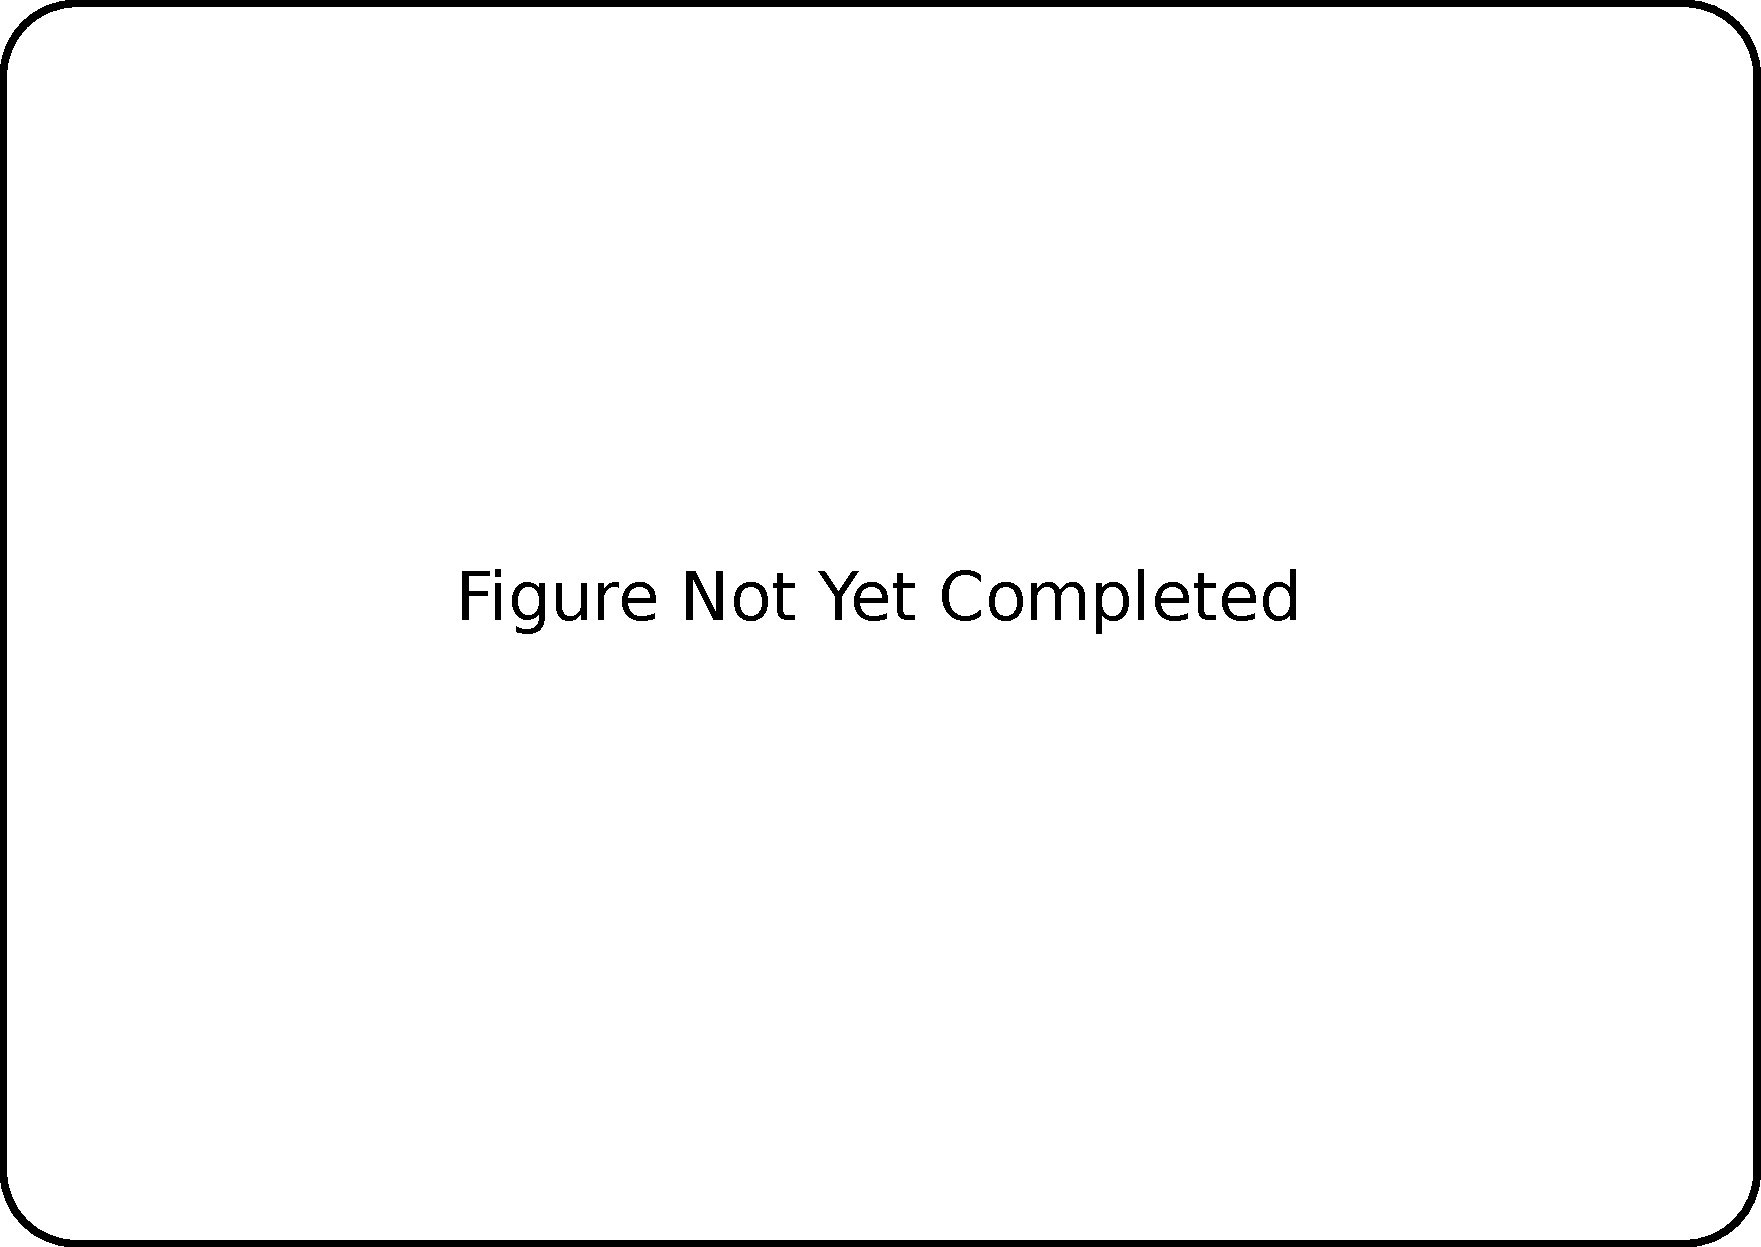
\includegraphics[width=4in]{introduction/not_finished.pdf}
\end{center}
\caption{Flow schematic for the PIC method. Need to make figure}
\label{fig:pic_flowchart}
\end{figure}


%%%%%%%%%%%%%%%%%%%%%%%%%%%%%%%%%%%% 
	\section{Motivation}
%%%%%%%%%%%%%%%%%%%%%%%%%%%%%%%%%%%%

	The PIC method is very good at modeling complicated plasma behaviour, however this method still relies on tracking a very large number of particles for good statistics. In order to achieve ``good'' statistics PIC codes employ millions to billions of particles, which means that these codes can require a very large amount of computation time for each timestep. Running millions of particles on a single processor for hundreds of timesteps is not really feasible, it simply takes too long to compute a solution. 
	
	One way to reduce the total run time of PIC codes is to parallelize them. Since PIC codes operate on the fact that the potential changes little over the course of a single timestep, each particle can be assumed to be independent of its neighbors. This leads to a situation that is trivially parallel. In theory a machine with a million processors could run every particle on a seperate processor. This is of course assuming that the majority of the computational complexity lies in moving the particles and that comunication between processors is very fast.  


%%%%%%%%%%%%%%%%%%%%%%%%%%%%%%%%%%%%
		\subsection{GPUs vs CPUs}
%%%%%%%%%%%%%%%%%%%%%%%%%%%%%%%%%%%%
	The ideal computing system for a particle in cell code should have a large number of relatively simple processors with very low communication costs. Traditional CPUs are just the oposite of this. CPUs tend to have 4-8 complicated processors that are very good at performing large operations on small sets of data, but very slow when it comes to communicating between multiple processors. CPUs are designed to be able to actively switch tasks on the fly. This makes them very good at simultaneously running web-browser, decoding a video, and playing a video game. However, this flexiblity requires a large number of cycles to switch between tasks, and a large amount of cache to store partially completed tasks.

Graphical processing units, or GPUs, forgoe the flexibility of CPUs in favor of more raw processing capability. Reducing the size of the cache and employing single instruction multiple data (SIMD) parallelism allows GPU manufactures to combine hundreds of processors on a single chip. In order to supply enough data to keep hundreds of processors GPUs also have a very large data channel between the processors and DRAM. All of these features are chosen to create a math processor that excels at tasks where each processor operates on data that is invisible to the other processors. These features give GPUs a significant raw floating point performance advantage over CPUs as seen in figure \ref{fig:gpu_vs_cpu}. 


\begin{figure}
\begin{center}
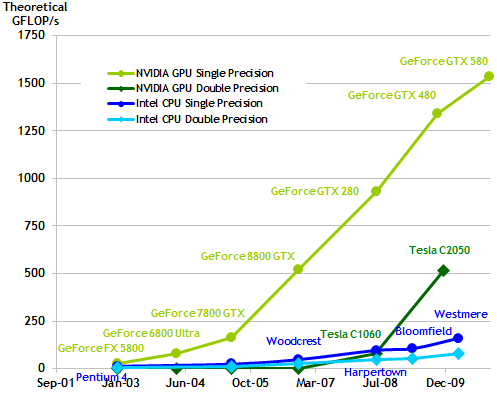
\includegraphics[width=4in]{introduction/gpu_vs_cpu.png}
\end{center}
\caption{Performance comparison of GPUs vs CPUs.}
\label{fig:gpu_vs_cpu}
\end{figure}

The hardware in GPUs is tailored to excel at performing tasks such as ray-tracing, which is very similar to particle moving. Therefore it is by no means unreasonable to conclude that GPUs can be very good PIC code processors. The advantages that GPUs have over CPUs for scientific computing include:

\begin{itemize}
	\item Higher performance per cost.
	\item Higher performance per watt.
	\item Easier to upgrade.
	\item GPUs still improving with Moore's law.
\end{itemize}

All of which are observed when comparing the CPU and GPU versions of the same PIC code. While these advantages are very promising there are also several disadvantages to GPU computing:

\begin{itemize}
	\item Increased code complexity.
	\item Smaller memory space.
	\item Smaller cache.
	\item Slow communication between CPU and GPU.
	\item Most developed GPU language is an extension of C.
	\item Algorithms can be very dependent on hardware configuration.
\end{itemize}

The key to developing efficient PIC algorithms that utilize GPUs lies in balancing the work between the two architectures. Some operations will be easier to implement on the CPU and be just as fast as the GPU while others will be significantly faster on the GPU. Partitioning the code between the different architectures begins to outline a very important aspect of parallel computing, multiple levels of parallelism.

%%%%%%%%%%%%%%%%%%%%%%%%%%%%%%%%%%%%
	\section{Multiple Levels of Parallelism}
%%%%%%%%%%%%%%%%%%%%%%%%%%%%%%%%%%%%
	Currently most parallelization is done by dividing up a task between a bunch of threads on different CPUs, and using an interface such as MPI to allow those threads to communicate. This network of threads has a master node, usually node 0, which orchestrates the communication between the other nodes. This is analgous to how a single CPU-GPU system operates. The CPU is the ``Master'' and serves as a communication hub for groups of execution threads on the GPU called thread blocks. Each thread block is itself a cluster of threads that can communicate through a memory space aptly named ``shared memory''.

\begin{figure}
\begin{center}
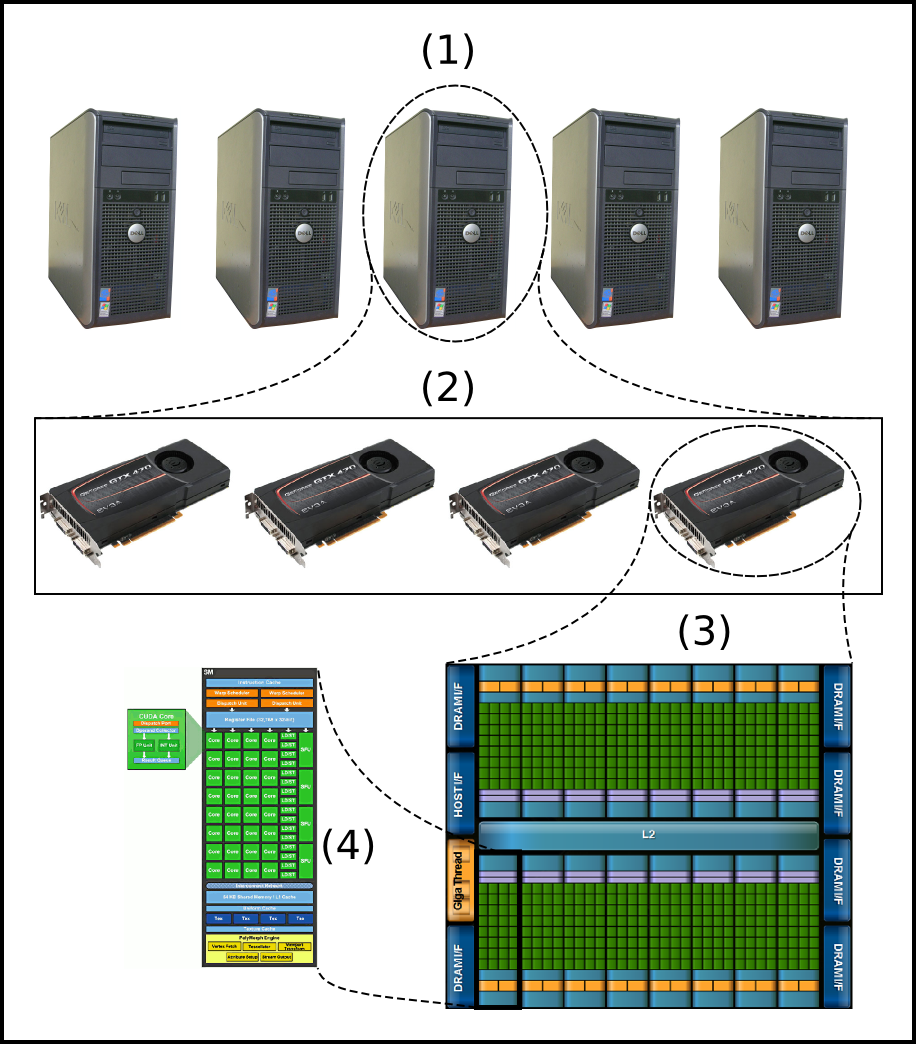
\includegraphics[width=5in]{introduction/multi_parallel.png}
\end{center}
\caption{Multiple levels of parallelism. (1) Cluster of systems communicating through a LAN. (2) Multiple GPUs per system communicating through system DRAM. (3) Multiple streaming multiprocessors per GPU execute thread-blocks and communicate through GPU global memory. (4) Multiple cuda cores per multiprocessor execute thread-warps and communicate through on chip shared memory. }
\label{fig:multiparallel}
\end{figure}

%%%%%%%%%%%%%%%%%%%%%%%%%%%%%%%%%%%%
		\subsection{Parallelization Opportunities in PIC Codes}
%%%%%%%%%%%%%%%%%%%%%%%%%%%%%%%%%%%%

\begin{figure}
\begin{center}
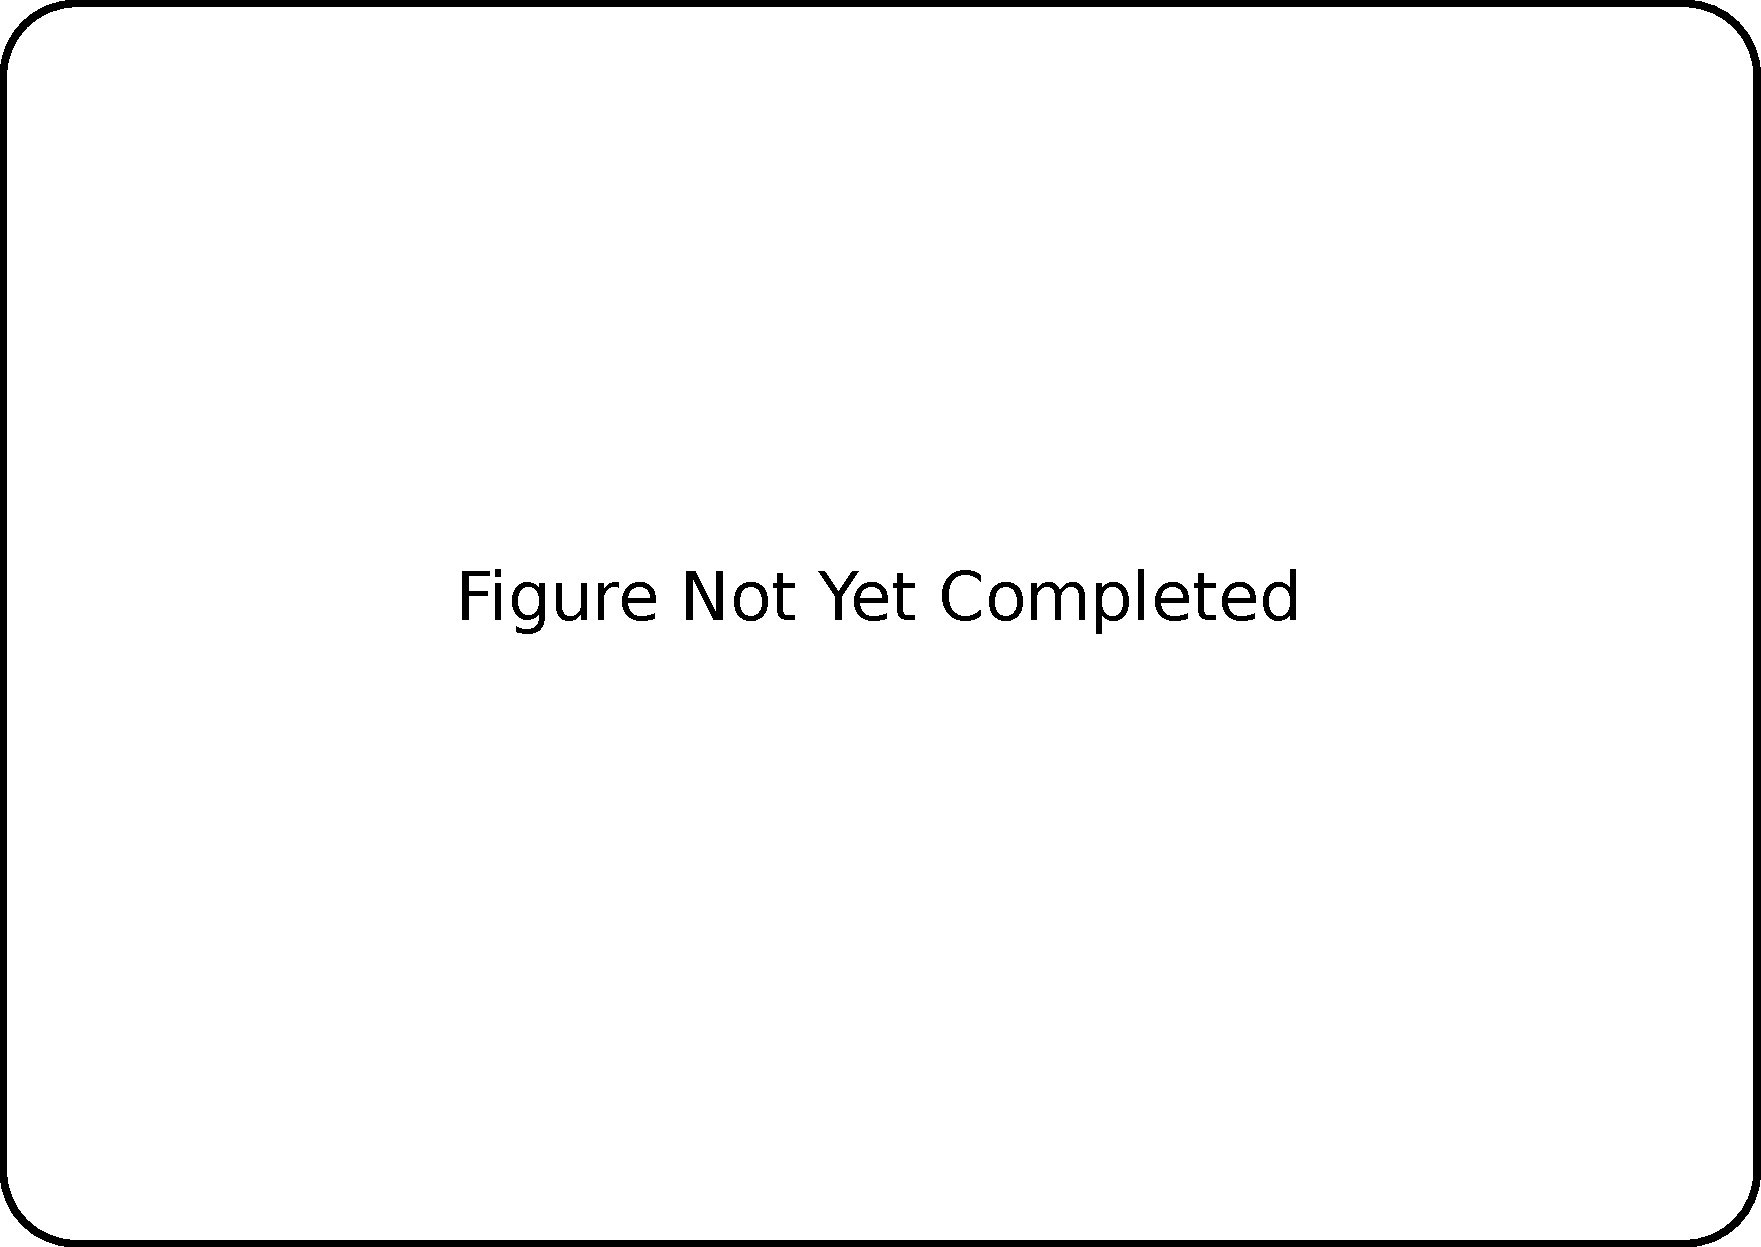
\includegraphics[width=4in]{introduction/not_finished.pdf}
\end{center}
\caption{Flow schematic for the PIC method with parallelizable steps highlighted. Need to make figure}
\label{fig:pic_flowchart_parallel}
\end{figure}

	
	\section{Overview of sceptic3D}











%%%%%%%%%%%%%%%%%%%%%%%%%%%%%%%%%%%%
	\chapter{Sceptic3D}
%%%%%%%%%%%%%%%%%%%%%%%%%%%%%%%%%%%%
Now that Sceptic3D is three dimensional hybrid PIC code specifically designed to solve the problem of ion flow past a negativley biased sphere in a uniform magnetic field. The current version of the code was derivied from the 2D/3v code SCEPTIC which was originally written by Hutchinson \cite{Hutchinson2002,Hutchinson2003,Hutchinson2005,Hutchinson2006}.



%%%%%%%%%%%%%%%%%%%%%%%%%%%%%%%%%%%%
		\section{Basic Code Structure}
%%%%%%%%%%%%%%%%%%%%%%%%%%%%%%%%%%%%
\begin{figure}
\begin{center}
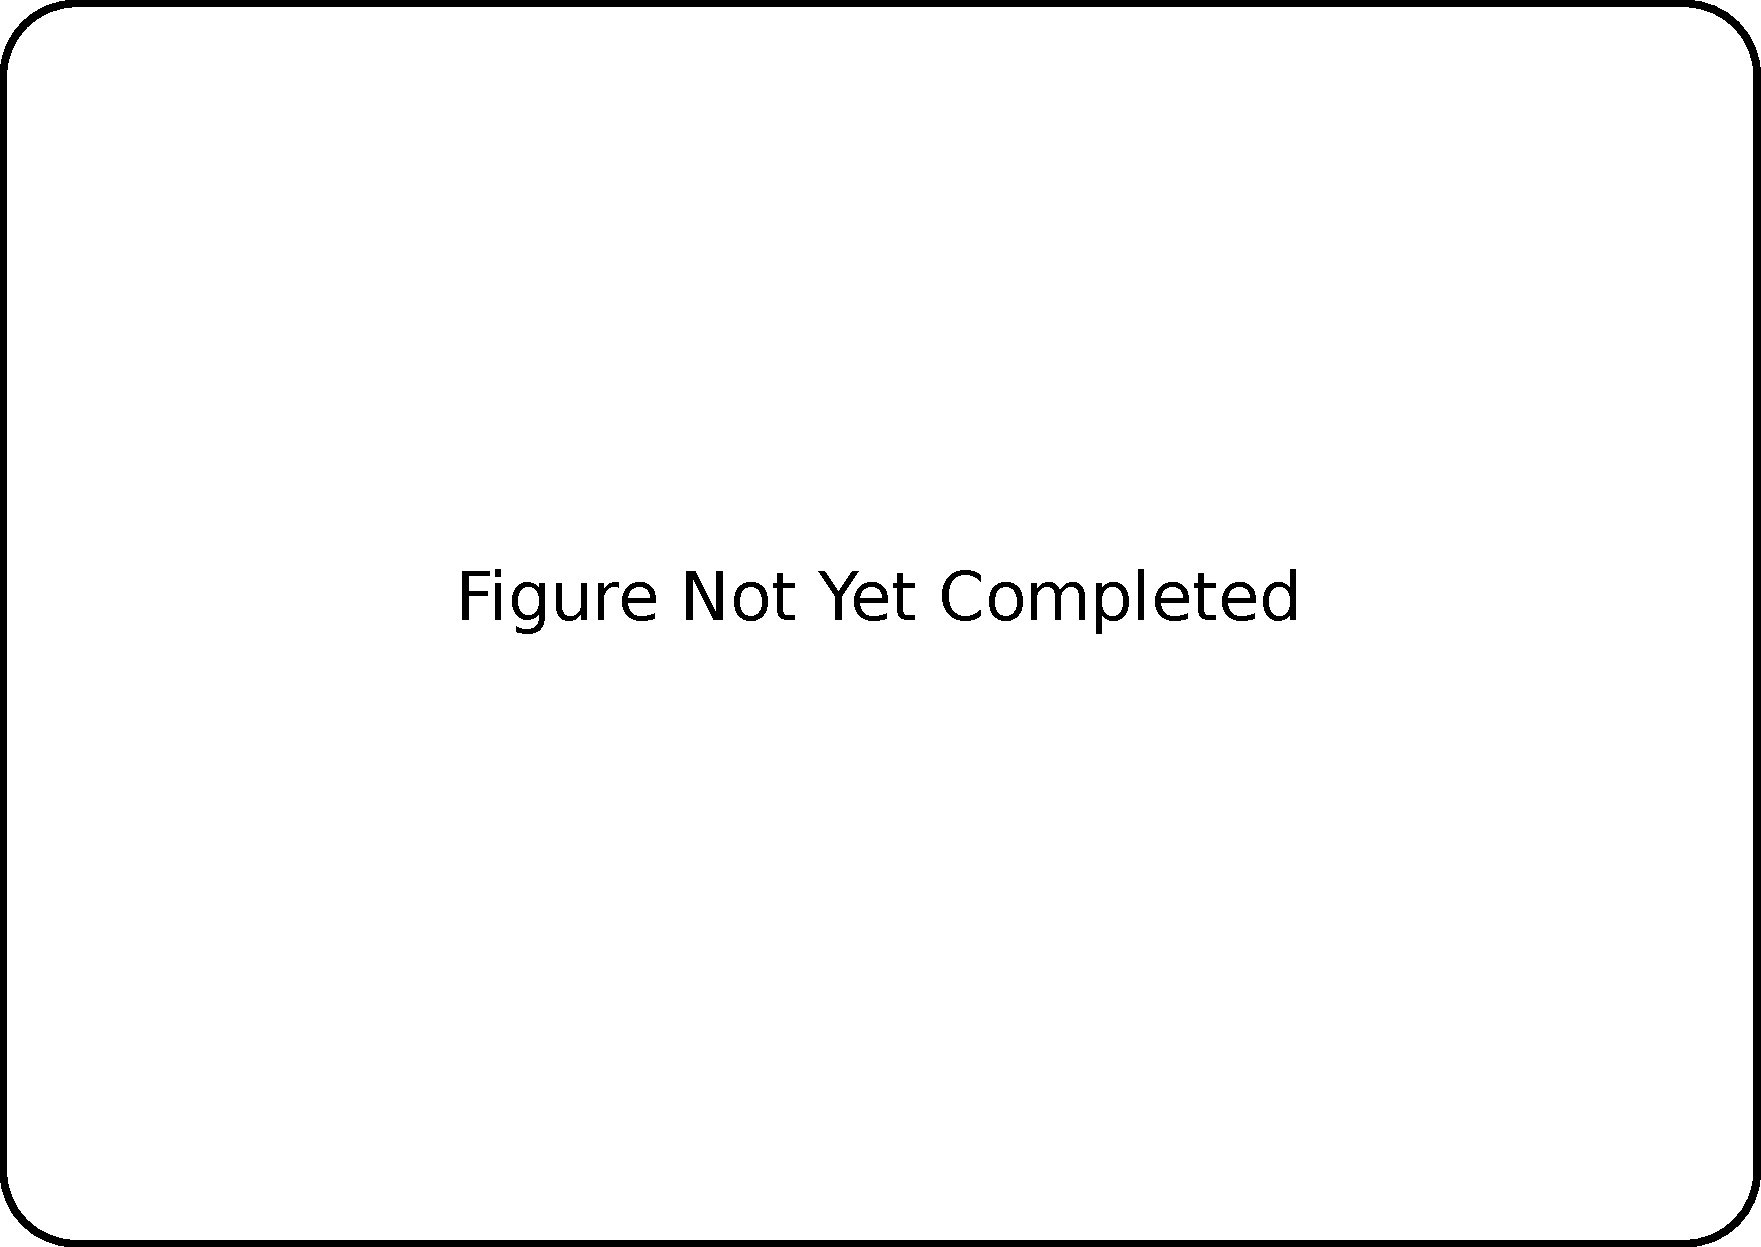
\includegraphics[width=4in]{introduction/not_finished.pdf}
\end{center}
\caption{Flow schematic for the PIC method with sceptic subroutine names Need to make figure}
\label{fig:pic_flowchart_sceptic}
\end{figure}
		
		\subsection{Charge Assign Details}
		
		\subsection{Poisson Solve Details}
		
		\subsection{Particle Advancing Details}
		

		\section{CPU Code Profiling}

	\section{Overview of sceptic3Dgpu Goals}

		\subsection{Main Routines}

		\subsection{Supporting Routines}

		\subsection{Challenges to overcome}
















%% This is an example first chapter.  You should put chapter/appendix that you
%% write into a separate file, and add a line \include{yourfilename} to
%% main.tex, where `yourfilename.tex' is the name of the chapter/appendix file.
%% You can process specific files by typing their names in at the 
%% \files=
%% prompt when you run the file main.tex through LaTeX.
\chapter{Design Options}
\label{ch:design}

GPU architecture is significantly different than that of a CPU, and a high performance PIC code on a GPU will look a lot different from its CPU equivalent. Memory access patterns, cache behavior, thread communication, and thread workload all have significant impacts on the performance of GPU codes. This means that porting an existing PIC code to the GPU is not straightforward, the data structures and algorithms will likely be different from the original serial code. 

Performance is just one facet of code design, maintaining separate CPU and GPU versions of the same code presents additional problems. Maximizing the amount of code that can be used for both the CPU and GPU versions also helps minimize the number of bugs and can help make the code easier to read. If a new feature is desired, then two different implementations of that feature must be written and debugged. From the lazy programmers perspective this is to be avoided as much as possible. Therefore, it is very important that the GPU version of the code utilize as much of the CPU code as possible. This means that interoperability between the CPU and GPU code must be both efficient and fast. 

Performance and maintenance are the two key issues that were considered when designing SCEPTIC3DGPU. Some of these issues have been investigated previously, although this area of research is still in its infancy. To make matters worse, the specific techniques used are rapidly evolving with every new generation of graphics card. It is unlikely that the pace of GPU hardware evolution will slow in the near future. Spending large amounts of time optimizing algorithms for the current generation of hardware is inadvisable, and therefore the design of the code should focus on utilizing techniques that emphasize underlying principles of GPU design or utilize library functions that will be optimized for each generation of hardware. 

The goal of this chapter is to outline various design options for implementing various steps of the PIC algorithm on GPUs and explore the pros and cons of each option. Solutions used by other researchers will be outlined and evaluated based on their applicability to SCEPTIC3D and to PIC codes in general. To accelerate these evaluations, several basic comparison codes were implemented, as well as a simple 3D sandbox GPUPIC code.

%%%%%%%%%%%
%This means that separate CPU and GPU versions of the code must be maintained depending on the features desired for each architecture. Maintaining two separate versions of a code and as such it is important that the focus of GPU PIC code development be focused on steps of the PIC algorithm that are the most computationally intensive. Steps should be taken during the development to 


%For a serial or even MPI PIC implementations there is enough memory that each thread can have a separate copy of the grid and only need to talk to one another after chugging through a massive list of particles. In these cases the communications costs are negligible compared to the computations performed by each thread. On the GPU the situation is a lot different. Instead of a few threads doing lots of work you have a lot of threads doing little work. 
%%%%%%%%%%%
%%%%%%%%%%%%%%%%%%%%%%%%%%%%%%%%%%%%
	\section{GPUPIC Sandbox}
%%%%%%%%%%%%%%%%%%%%%%%%%%%%%%%%%%%%
The first step in the development of SCEPTIC3DGPU was to create a very simple, generalized pic code that performed the major steps of the PIC algorithm and implement it in \gls{gls:CUDA}. This simple code, we'll call it GPUPIC\_testbed is designed without making any assumptions about the physics of the system. GPUPIC\_testbed operates in Cartesian coordinates with periodic boundary conditions. We do not really care too much about the field solve since in the serial version it takes a very small amount of time compared to the particle advance and charge assign steps. By recognizing the low priority of the field solve we really only need to characterize the performance of the following steps:


\begin{enumerate}\itemsep0pt \parskip0pt \parsep0pt
\item Read the particle data
\item Read the Potential data for that particle
\item Move the particle
\item Write the new particle data to the particle list
\item Interpolate Charge to Mesh
\item Repeat
\end{enumerate}



The first implementation of this code was very naive. The only real difference from a serial version was the density array update, which used atomic updates on global memory in order to prevent memory collisions between multiple threads. Other than that the code boiled down to unrolling the loop over all of the particles into one particle per thread. The runtime breakdown of this code for a $32^3$ grid and 4.2 million particles is shown in figure \ref{fig:GPUPIC_basetime}.


\begin{figure}
\begin{center}
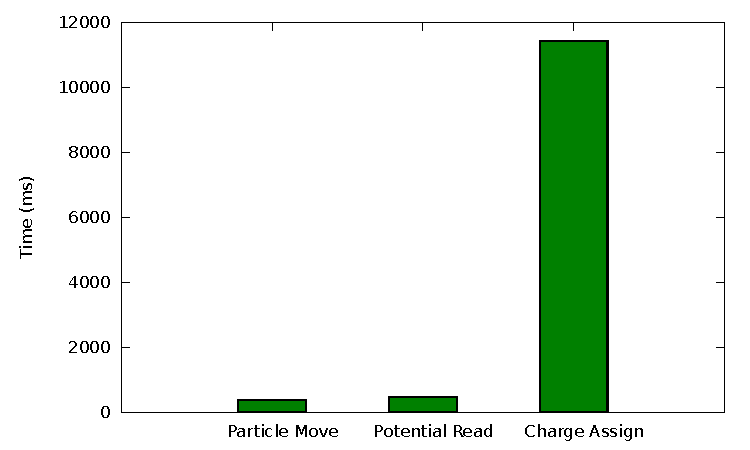
\includegraphics[width=5in]{design/sandbox_run_histo.pdf}
\end{center}
\caption[Sandbox GPUPIC Code Profile]{Total Execution times for 100 iterations of the key steps of the move kernel. The charge assign dominates the run time by a very large margin.}
\label{fig:GPUPIC_basetime} 
\end{figure}



As shown by the figure, the particle move and the potential read are very similar, but the charge assign is very slow. Determining how the charge assign can be better adapted to the GPU is the first major challenge. Several ways of dealing with the issue of the charge assign will be discussed in the following section. The other issues that will be discussed in this chapter are:

\begin{itemize}\itemsep0pt \parskip0pt \parsep0pt
\item Particle Data Structure: Is it better to use an Array of structures, like the fortran code, or a Structure of Arrays?
\item How do we handle divergent processes in the advancing routine, such as losses, reinjections, and collisions?
\item At what point does the field solve become a dominant cost?
\item Are there any new issues that arise from solutions to the other issues?
\end{itemize}

%%%%%%%%%%%%%%%%%%%%%%%%%%%%%%%%%%%%
	\section{Charge Assign}
%%%%%%%%%%%%%%%%%%%%%%%%%%%%%%%%%%%%

There are two different ways to approach the charge assign, one in which information is ``pulled" from the particles by the mesh vertices, and one in which data is ``pushed" by the particles to the mesh vertices. Let G represent a grid of domain D of dimension d comprised of all mesh vertices $v_s  \in \mathrm{D}$. We can define some distribution function $f(v_s)$ at each of the mesh vertices which is the sum of some function $\mathrm{K}(v_s,p_i)$, where $p_i$ is the position of particle $i$. 
$\mathcal{P}(v_s)$ is a list of all particles contributing to vertex $v_s$ and $\mathcal{V}(p_i)$ is the list of all vertices that particle $p_i$ contributes to.
Given these definitions the algorithms for the particle pull and particle push method are algorithms \ref{alg:particle_pull} and \ref{alg:particle_push} respectively. 

\begin{algorithm}
	\begin{algorithmic}
		\STATE // Loop over the vertices first
		\FORALL{$\mathrm{vertex} \: v_s \in G$}
			\STATE find $\mathcal{P}(v_s)$
			\STATE $\mathrm{f}(v_s) \leftarrow 0$
			\FORALL{$p_i \in \mathcal{P}(v_s)$}
			\STATE $\mathrm{f}(v_s) \leftarrow \mathrm{f}(v_s) + \mathrm{K}(v_s,p_i)$
			\ENDFOR
		\ENDFOR
	\end{algorithmic}
	\caption[Particle Pull Method of charge deposition.]{Particle Pull Method of charge deposition. From Stantchev et al. \cite{Stantchev2008}}
	\label{alg:particle_pull}
\end{algorithm}

\begin{algorithm}
	\begin{algorithmic}
		\FORALL{$\mathrm{vertex} \: v_s \in G$}
			\STATE $\mathrm{f}(v_s) \leftarrow 0$
		\ENDFOR
		\STATE // Loop over all particles
		\FORALL{$\mathrm{particle} \: p_i \in \mathrm{D}$}
			\STATE find $\mathcal{V}(p_i)$ // The vertices that particle $p_i$ will contribute to
			\FORALL{$v_s \in \mathcal{V}(p_i)$}
				\STATE $\mathrm{f}(v_s) \leftarrow \mathrm{f}(v_s) + \mathrm{K}(v_s,p_i)$
			\ENDFOR
		\ENDFOR
	\end{algorithmic}
	\caption[Particle Push Method of charge deposition.]{Particle Push Method of charge deposition. From Stantchev et al. \cite{Stantchev2008}}
	\label{alg:particle_push}
\end{algorithm}

As pointed out by Stantchev \cite{Stantchev2008}, each method has its advantages and disadvantages. For an algorithm consisting of N particles and k grid vertices the advantages and disadvantages are as follows:

The particle pull method
\begin{itemize}
\item requires $\mathcal{O}(2^dN + k)$ read write operations
\item $\mathcal{P}(v_s)$ is expensive to retrieve dynamically unless particles are organized
\end{itemize}

The particle push method
\begin{itemize}
\item requires $\mathcal{O}((2^d+1)N)$ read/write operations
\item $\mathcal{V}(p_i)$ is easily computed dynamically from the particles coordinates
\end{itemize}


\begin{figure}
\begin{center}
% Turing Machine
% Author: Sebastian Sardina
%\documentclass[a4paper,10pt]{article}
%\usepackage[usenames,dvipsnames]{xcolor}
%\usepackage{tikz}
%\usetikzlibrary{chains,fit,shapes}
%\begin{document}

\noindent
\begin{tikzpicture}
		\tikzstyle{every path}=[very thick]

		\edef\sizetape{1.0cm}
		\tikzstyle{tmtape}=[draw,minimum size=\sizetape]
		\tikzstyle{tmtape1}=[draw,minimum size=0.4cm]
		\tikzstyle{tmhead}=[arrow box,draw,minimum size=0.4cm,arrow box
		arrows={east:.25cm}]

		\tikzstyle{cfill1}=[fill=Purple]
		\tikzstyle{cfill2}=[fill=SkyBlue]
		\tikzstyle{cfill3}=[fill=Maroon]
		\tikzstyle{cfill4}=[fill=Emerald]

\node [shift={(-1.0cm,-2cm)}]
	{
		\begin{tikzpicture}[remember picture]



					\begin{scope}[start chain=2 going below,start chain=1 going right,node distance=-0.15mm] at (current page.north west)
						 \node [on chain=2,yshift=0.5cm] {Particle Stream};
						 \node [on chain=1,tmtape1,draw=none,xshift=-5cm] {$\ldots$};
						 \node [on chain=1,tmtape1,cfill1] (input) {};
						 \node [on chain=1,tmtape1,cfill4] (i0) {};
						 \node [on chain=1,tmtape1,cfill3] (i3) {};
						 \node [on chain=1,tmtape1,cfill2] (i4) {};
						 \node [on chain=1,tmtape1,cfill1] (i5) {};
						 \node [on chain=1,tmtape1,cfill4] {};
						 \node [on chain=1,tmtape,draw=none] {$\ldots$};
						 \node [on chain=1,tmtape1,cfill3] (i6) {};
						 \node [on chain=1,tmtape1,cfill2] (i7) {};
						 \node [on chain=1,tmtape1,cfill1] (i8) {};
						 \node [on chain=1,tmtape1,cfill3] (i9) {};
						 \node [on chain=1,tmtape1,cfill4] (i11) {};
						 \node [on chain=1,tmtape,draw=none] {$\ldots$};
						 \node [on chain=1,tmtape1,cfill4] (i11) {};
						 \node [on chain=1,tmtape1,cfill3] (i12) {};
						 \node [on chain=1,tmtape1,cfill2] (i13) {};
						 \node [on chain=1,tmtape1,cfill4] (i16) {};
						 \node [on chain=1,tmtape1,cfill1] (i17) {};
						 \node [on chain=1,tmtape,draw=none] {$\ldots$};
						 
					\end{scope}

		\node [tmhead,yshift=-0.45cm] at (input.south) (head1) {$T_1$};
		\node [tmhead,yshift=-0.45cm] at (i6.south) (head2) {$T_2$};
		\node [tmhead,yshift=-0.45cm] at (i11.south) (head3) {$T_3$};

		
		\footnotesize
		\node [xshift=-3cm,yshift=-5cm] (a1)
			{\begin{tikzpicture}[remember picture]
			\begin{scope}[start chain=1 going right,start chain=3 going down,start chain=2 going right,node distance=-1.0mm]

				 \node [on chain=1,tmtape,cfill1] (j1) {j};
				 \node [on chain=1,tmtape,cfill2] (j2) {j+1};
				 \node [on chain=2,tmtape,cfill3,yshift=-.985cm] at (j1) (j3) {j+2};
				 \node [on chain=2,tmtape,cfill4] (j4) {j+3};
				 \node [on chain=3,yshift=-0.75cm,xshift=-0.5cm] at (j4) {Array 1};  

			\end{scope}
			\end{tikzpicture}
			};

		\node [shift={(3cm,0cm)}] at (a1) (a2)
			{\begin{tikzpicture}[remember picture]
			\begin{scope}[start chain=1 going right,start chain=3 going down,start chain=2 going right,node distance=-1.0mm]
   
				 \node [on chain=1,tmtape,cfill1] (j5) {j};
				 \node [on chain=1,tmtape,cfill2] (j6) {j+1};
				 \node [on chain=2,tmtape,cfill3,yshift=-.985cm] at (j5) (j7) {j+2};
				 \node [on chain=2,tmtape,cfill4] (j8) {j+3};
				 \node [on chain=3,yshift=-0.75cm,xshift=-0.5cm] at (j8) {Array 2};  

			\end{scope}
			\end{tikzpicture}
			};

		\node [shift={(3cm,0cm)}] at (a2)
			{\begin{tikzpicture}[remember picture]
			\begin{scope}[start chain=1 going right,start chain=2 going right,start chain=3 going down,node distance=-1.0mm]

				   
				 \node [on chain=1,tmtape,cfill1] (j9) {j};
				 \node [on chain=1,tmtape,cfill2] (j10) {j+1};
				 \node [on chain=2,tmtape,cfill3,yshift=-.985cm] at (j9) (j11) {j+2};
				 \node [on chain=2,tmtape,cfill4] (j12) {j+3};
				 \node [on chain=3,yshift=-0.75cm,xshift=-0.5cm] at (j12) {Array 3};  

			\end{scope}
			\end{tikzpicture}
			};





			\path[->] (head1) edge [bend right] (j1);	
			\path[->] (head2) edge [out=-90, in=180] (j7);
			\path[->] (head3) edge [out=-90, in=45] (j12);	

			\end{tikzpicture}
	};
\end{tikzpicture}
%\end{document}


\end{center}
\caption[Charge Assign using MPI]{Every thread $T_i$ reads in some random subset of the particle list and records the contributions of its subset to a copy of the density array. Once all threads have processed their respective sub-lists a prefix sum is used to condense all of the contributions to a single array.}
\label{fig:mpi_chargeassign}
\end{figure}

The challenge of the charge assign is that with a completely random particle list any given particle can contribute to any element of the grid. For parallel implementations using \gls{ac:mpi}, the solution, shown in figure \ref{fig:mpi_chargeassign}, involves setting aside enough memory to store the entire domain for each thread. Each thread deals with a subset of the particle list and tallies up the contributions of that list to some array in memory private to a single thread. Once every thread has recorded the contributions from their subset of the particle list a parallel reduction is performed in order to quickly sum up the contributions from all threads. 


Applying a similar technique on the GPU would require massive amounts of memory. Memory is a valuable commodity on the GPU, and ideally we want to use as much of it as possible for the particle list. We need to determine a way in which we only need one copy of the density array in global memory. The problem is that if two threads attempt to update the same element in the density array at the same time, such as in figure \ref{fig:atomic_memory_collisions}, a memory conflict occurs and only one threads contribution will be recorded. 

\begin{figure}
\begin{center}
% Turing Machine
% Author: Sebastian Sardina
%\documentclass[a4paper,10pt]{article}
%\documentclass{standalone}

%\begin{document}
\begin{tikzpicture}
\tikzstyle{every path}=[very thick]

\edef\sizetape{1.0cm}
\tikzstyle{tmtape}=[draw,minimum size=\sizetape]
\tikzstyle{tmtape1}=[draw,fill=Gray,minimum size=\sizetape]
\tikzstyle{tmhead}=[arrow box,draw,minimum size=.5cm,arrow box
arrows={east:.25cm, west:0.25cm}]

\tikzstyle directed=[postaction={decorate,decoration={markings,
    mark=at position .65 with {\arrow[arrowstyle]{stealth}}}}]

\tikzstyle arrowstyle=[scale=1]

\tikzstyle{cfill1}=[fill=Purple]
\tikzstyle{cfill2}=[fill=SkyBlue]
\tikzstyle{cfill3}=[fill=Maroon]
\tikzstyle{cfill4}=[fill=Emerald]

%% Draw TM tape
\begin{scope}[start chain=1 going right,node distance=-0.15mm]
    \node [on chain=1,tmtape,draw=none] {$\ldots$};
    \node [on chain=1,tmtape1] (input) {};
    \node [on chain=1,tmtape1,cfill1] (i0) {i};
    \node [on chain=1,tmtape1,cfill1] (i1) {i+1};
    \node [on chain=1,tmtape1,cfill2] (i2) {i+2};
    \node [on chain=1,tmtape1,cfill3] (i3) {i+3};
    \node [on chain=1,tmtape1,cfill4] (i4) {i+4};
    \node [on chain=1,tmtape1,cfill4] (i5) {i+5};
    \node [on chain=1,tmtape1] {};
    \node [on chain=1,tmtape,draw=none] {$\ldots$};
    \node [on chain=1] {\textbf{Particle stream}};

\end{scope}
\begin{scope}
[shift={(1.25cm,-3cm)},start chain=1 going right,node distance=-0.15mm]
    \node [on chain=1,tmtape,draw=none] {$\ldots$};
    \node [on chain=1,tmtape] (input) {};
    \node [on chain=1,tmtape,cfill1] (j1) {j};
	 \node [on chain=1,tmtape,cfill2] (j2) {j+1};
	 \node [on chain=1,tmtape,cfill3] (j3) {j+2};
	 \node [on chain=1,tmtape,cfill4] (j4) {j+3};
    \node [on chain=1,tmtape] {};
    \node [on chain=1,tmtape,draw=none] {$\ldots$};
    \node [on chain=1] {\textbf{Density Array}};
	

		

	%\draw[directed,dashed,red] (i0) -- (j1);	
	%\draw[directed,dashed,red] (i1) -- (j1);	
	%\draw[directed,dashed] (i2) -- (j2);
	%\draw[directed,dashed] (i3) -- (j3);	
	%\draw[directed,dashed,red] (i4) -- (j4);
	%\draw[directed,dashed,red] (i5) -- (j4);	
	\path[dashed,red] (i0) edge [directed,out=-90, in=90] (j1);	
	\path[dashed,red] (i1) edge [directed,out=-90, in=90] (j1);	
	\path[dashed] (i2) edge [directed,out=-90, in=90] (j2);
	\path[dashed] (i3) edge [directed,out=-90, in=90] (j3);	
	\path[dashed,red] (i4) edge [directed,out=-90, in=90] (j4);
	\path[dashed,red] (i5) edge [directed,out=-90, in=90] (j4);	
	%\draw[color=red] (j4)	circle (0.7cm);
	%\draw[color=red] (j1)	circle (0.7cm);

	\path ++(j1)++(90:0.6cm) coordinate (c1);
	\path ++(j4)++(90:0.6cm) coordinate (c2);
	\path ++(j4)++(4cm,1.25cm) node [red] {\textbf{Memory Conflicts}};
	\path ++(j4)++(2cm,1.25cm) coordinate (c4);
	\path ++(j4)++(1.5cm,1.25cm) coordinate (c3);

	\draw[->,color=red] (c1) -- (c3) -- (c4);
	\draw[->,color=red] (c2) -- (c3) -- (c4);
\end{scope}


\end{tikzpicture}
%\end{document}


\end{center}
\caption[Density Accumulation Memory Collisions]{One thread is launched for every particle. Conflicts arise whenever two threads attempt to update the same element of the density array at the same time. Without atomic operations only one threads contribution would be counted.  Atomic operations can be used in order to ensure that every thread's contribution to the density is accounted for. However, when a memory conflict occurs between threads using atomic operations the execution becomes serialized, significantly reducing the operation's efficiency.}
\label{fig:atomic_memory_collisions}
\end{figure}

In the sandbox PIC code we used atomic operations to prevent memory collisions during the charge assign. Looking back at figure \ref{fig:GPUPIC_basetime} we notice that the charge assign step constitutes about 93\% of the total runtime.  Unfortunately this poor performance is a result of serialization caused by the atomic updates. Additionally, since the grid is far too large to fit in \emph{\_\_shared\_\_} memory these updates must be performed on device global memory, which has much higher latency and lower bandwidth. When a thread attempts to update a value in memory and finds that it is locked it must then repeat the process until it succeeds. Every failed update represents an additional slow global memory access that is essentially wasted.




However, if we can ensure that a thread knows that every particle it reads in will only contribute to one element of the grid, then the operation that the thread has to perform is a simple sum.
Since this thread knows that every particle it sees will only contribute to a single value, each thread requires only enough memory for their single value. 
When it comes time for all of the threads to contribute to the final result each thread provides the full answer for a single element. 
This is essentially the particle pull method described in algorithm \ref{alg:particle_pull} without the need to to retrieve $\mathcal{P}(v_s)$ dynamically. An illustration of this method is shown in figure \ref{fig:one_thread_per_cell}.
One of the main benefits to this method is that it significantly reduces the memory requirements of each thread but imposes the constraint that a thread is given only particles that exist within a thread's domain. This additional constraint will be addressed in section \ref{sec:plist_sort_design}. 

\begin{figure}
\begin{center}
% Turing Machine
% Author: Sebastian Sardina
%\documentclass[a4paper,10pt]{article}
%\usepackage[usenames,dvipsnames]{xcolor}
%\usepackage{tikz}
%\usetikzlibrary{chains,fit,shapes}
%\begin{document}


\begin{tikzpicture}\noindent

\node [shift={(0cm,0cm)}]
	{
		\begin{tikzpicture}[remember picture]
\tikzstyle{every path}=[very thick]

\edef\sizetape{1.0cm}
\tikzstyle{tmtape}=[draw,minimum size=\sizetape]
\tikzstyle{tmtape1}=[draw,minimum size=\sizetape]
\tikzstyle{tmhead}=[arrow box,draw,minimum size=0.8cm,arrow box
arrows={east:.25cm}]

\tikzstyle{cfill1}=[fill=Purple]
\tikzstyle{cfill2}=[fill=SkyBlue]
\tikzstyle{cfill3}=[fill=Maroon]
\tikzstyle{cfill4}=[fill=Emerald]



%% Draw Density Array
\begin{scope}[start chain=1 going right,node distance=-0.15mm]
    \node [on chain=1,tmtape,draw=none] {$\ldots$};
    \node [on chain=1,tmtape,fill=Gray] (input) {};
    \node [on chain=1,tmtape,cfill1] (j1) {j};
	 \node [on chain=1,tmtape,cfill2] (j2) {j+1};
	 \node [on chain=1,tmtape,cfill3] (j3) {j+2};
	 \node [on chain=1,tmtape,cfill4] (j4) {j+3};
    \node [on chain=1,tmtape,fill=Gray] {};
    \node [on chain=1,tmtape,draw=none] {$\ldots$};
    \node [on chain=1] {\textbf{Density Array}};


\end{scope}

\begin{scope}[shift={(-1cm,-4cm)},start chain=1 going right,node distance=-0.15mm]

    \node [on chain=1,tmtape,draw=none] {$\ldots$};
    \node [on chain=1,tmtape1,cfill1] (input) {i};
    \node [on chain=1,tmtape1,cfill1] (i0) {i+1};
	 \node [on chain=1,tmtape,draw=none] {$\ldots$};
    \node [on chain=1,tmtape1,cfill2] (i1) {i+2};
    \node [on chain=1,tmtape1,cfill2] (i2) {i+3};
	 \node [on chain=1,tmtape,draw=none] {$\ldots$};
    \node [on chain=1,tmtape1,cfill3] (i3) {i+4};
    \node [on chain=1,tmtape1,cfill3] (i4) {i+5};
 	 \node [on chain=1,tmtape,draw=none] {$\ldots$};
    \node [on chain=1,tmtape1,cfill4] (i5) {i+6};
    \node [on chain=1,tmtape1,cfill4] {i+7};
    \node [on chain=1,tmtape,draw=none] {$\ldots$};
    \node [on chain=1] {\textbf{Particle stream}};
	
\end{scope}

\node [tmhead,yshift=0.45cm] at (input.north) (head1) {$T_1$};
\node [tmhead,yshift=0.45cm] at (i1.north) (head2) {$T_2$};
\node [tmhead,yshift=0.45cm] at (i3.north) (head3) {$T_3$};
\node [tmhead,yshift=0.45cm] at (i5.north) (head4) {$T_4$};
		

	\path[->] (head1) edge [out=90, in=-90] (j1);	
	\path[->] (head2) edge [out=90, in=-90] (j2);
	\path[->] (head3) edge [out=90, in=-90] (j3);	
	\path[->] (head4) edge [out=90, in=-90] (j4);	

	\end{tikzpicture}
	};
\end{tikzpicture}
%\end{document}


\end{center}
\caption[One thread per cell]{One thread per cell. Each thread $T_i$ is responsible for a subset of the particle list. Each subset of the particle list corresponds to a single element of the density array.}
\label{fig:one_thread_per_cell}
\end{figure}

Since the operation performed at the thread level is a simple sum there should be a way that an additional level of parallelization can be added, and turn the method shown in figure \ref{fig:one_thread_per_cell} into a hybrid of the push and pull methods. Further parallelization can be accomplished by replacing the sum with a parallel reduction. This method, illustrated in figure \ref{fig:one_cell_per_block} the particles are sorted into subsets according to which cell they are contributing to. Each subset of the particle list is assigned to a thread block, or multiple thread blocks, and read into \emph{\_\_shared\_\_} memory. Once the contributions from all of the particles in the subset have been read into an array in \emph{\_\_shared\_\_} memory a parallel reduction is performed to condense the array of values into a single value. In this method there are zero memory conflicts as each thread reading in data from the particle list has a private memory space in which to record the values it reads. 
This reduction method approaches the limit of how far the particle to mesh mapping can be parallelized, in which every thread must process only a single particle. In this limit, the time complexity of accumulating the contributions of $N$ particles to $D$ elements is $\mathcal{O}(log(N/D))$, if the particles are evenly distributed across each element. 

\begin{figure}
\begin{center}
% Turing Machine
% Author: Sebastian Sardina
%\documentclass[a4paper,10pt]{article}
%\usepackage[usenames,dvipsnames]{xcolor}
%\usepackage{ifthen}
%\usepackage{tikz}
%\usetikzlibrary{chains,fit,shapes}
%\begin{document}

\noindent
\begin{tikzpicture}
		\tikzstyle{every path}=[very thick]

		\edef\sizetape{1.0cm}
		\tikzstyle{tmtape}=[draw,minimum size=\sizetape]
		\tikzstyle{tmtape1}=[draw,minimum size=0.4cm]
		\tikzstyle{tmhead}=[arrow box,draw,minimum size=0.4cm,arrow box
		arrows={east:.25cm}]
		\tikzstyle{tmblock}=[arrow box,draw,minimum height=0.4cm,minimum width=2.4cm,arrow box
		arrows={east:.25cm}]

		\tikzstyle{cfill1}=[fill=Purple]
		\tikzstyle{cfill2}=[fill=SkyBlue]
		\tikzstyle{cfill3}=[fill=Maroon]
		\tikzstyle{cfill4}=[fill=Emerald]


\def\ji{}

\node [shift={(-1.0cm,-2cm)}]
	{
		\begin{tikzpicture}[remember picture]




					\begin{scope}[start chain=2 going below,start chain=1 going right,node distance=-0.15mm] at (current page.north west)
						 \node [on chain=2,yshift=0.5cm] {Particle Stream};
						 \node [on chain=1,tmtape1,draw=none,xshift=-5cm] {$\ldots$};
						 \node [on chain=1,tmtape1,cfill1] (input) {};
						 \node [on chain=1,tmtape1,cfill1] (i0) {};
						 \node [on chain=1,tmtape1,cfill1] (i3) {};
						 \node [on chain=1,tmtape1,cfill1] (i4) {};
						 \node [on chain=1,tmtape1,cfill1] (i5) {};
						 \node [on chain=1,tmtape1,cfill1] {};
						 \node [on chain=1,tmtape,draw=none] {$\ldots$};
						 \node [on chain=1,tmtape1,cfill2] (i6) {};
						 \node [on chain=1,tmtape1,cfill2] (i7) {};
						 \node [on chain=1,tmtape1,cfill2] (i8) {};
						 \node [on chain=1,tmtape1,cfill2] (i9) {};
						 \node [on chain=1,tmtape1,cfill2] (i10) {};
						 \node [on chain=1,tmtape1,cfill2] (i11) {};
						 \node [on chain=1,tmtape,draw=none] {$\ldots$};
						 \node [on chain=1,tmtape1,cfill3] (i12) {};
						 \node [on chain=1,tmtape1,cfill3] (i13) {};
						 \node [on chain=1,tmtape1,cfill3] (i14) {};
						 \node [on chain=1,tmtape1,cfill3] (i15) {};
						 \node [on chain=1,tmtape1,cfill3] (i16) {};
						 \node [on chain=1,tmtape1,cfill3] (i17) {};
						 \node [on chain=1,tmtape,draw=none] {$\ldots$};
						 
					\end{scope}
					\begin{scope}[yshift=-0.48cm,start chain=2 going below,start chain=1 going right,node distance=-0.15mm] at (current page.north west)
						 \node [on chain=1,tmtape1,draw=none,xshift=-4.88cm] (nodestare) {};
						 \node [on chain=1,tmtape1,draw=none] (i20) {};
						 \node [on chain=1,tmtape1,draw=none] (i21) {};
						 \node [on chain=1,tmtape1,draw=none] (i22) {};
						 \node [on chain=1,tmtape1,draw=none] (i23) {};
						 \node [on chain=1,tmtape1,draw=none] (i24) {};
						 \node [on chain=1,tmtape1,draw=none] (i25) {};
						 \node [on chain=1,tmtape,draw=none] {};
						 \node [on chain=1,tmtape1,draw=none] (i26) {};
						 \node [on chain=1,tmtape1,draw=none] (i27) {};
						 \node [on chain=1,tmtape1,draw=none] (i28) {};
						 \node [on chain=1,tmtape1,draw=none] (i29) {};
						 \node [on chain=1,tmtape1,draw=none] (i210) {};
						 \node [on chain=1,tmtape1,draw=none] (i211) {};
						 \node [on chain=1,tmtape,draw=none] {};
						 \node [on chain=1,tmtape1,draw=none] (i212) {};
						 \node [on chain=1,tmtape1,draw=none] (i213) {};
						 \node [on chain=1,tmtape1,draw=none] (i214) {};
						 \node [on chain=1,tmtape1,draw=none] (i215) {};
						 \node [on chain=1,tmtape1,draw=none] (i216) {};
						 \node [on chain=1,tmtape1,draw=none] (i217) {};
						 \node [on chain=1,tmtape,draw=none] {};
						 
					\end{scope}


		\node [tmblock,yshift=-0.25cm,anchor=west] at (input.south west) (head1) {Thread Block 1};
		\node [tmblock,yshift=-0.25cm,anchor=west] at (i6.south west) (head2) {Thread Block 2};
		\node [tmblock,yshift=-0.25cm,anchor=west] at (i12.south west) (head3) {Thread Block 3};
		
\def\reduceArray{{3,2,1}}
\def\shiftArray{{0.6cm,0.2cm,0.2cm}}
			\foreach \j in {3,...,5} {
				\pgfmathtruncatemacro{\k}{\j - 1}
				\pgfmathtruncatemacro{\d}{\j - 3}
				\pgfmathsetmacro{\shift}{\shiftArray[\d]}

				\foreach \l in {1,...,3}{

					\pgfmathtruncatemacro{\a}{6*\l - 5}
					\pgfmathtruncatemacro{\c}{\l}

					\foreach \i in {0,...,5}{

						\pgfmathtruncatemacro{\b}{\a + \i - 1}
						\pgfmathtruncatemacro{\bc}{\reduceArray[\d]}
						\ifthenelse{\i < \bc}{
						
						\node [tmtape1,cfill\l,yshift=-1.0cm,xshift=\shift] at (i\k\b) (i\j\b) {};}{}
					}
				}

			}

		\foreach \k in {0,6,12}{
			\foreach \i in {0,1,2} {


					\pgfmathtruncatemacro{\a}{\i + \k}
					\pgfmathtruncatemacro{\b}{2*\i + \k}
					\pgfmathtruncatemacro{\c}{\b + 1}
					\path[->] (i2\b) edge[in=90,out=-90] (i3\a);
					\path[->] (i2\c) edge[in=90,out=-90] (i3\a);
			}
		}
		\foreach \k in {0,6,12}{



			\foreach \i in {0} {


					\pgfmathtruncatemacro{\a}{\i + \k}
					\pgfmathtruncatemacro{\b}{2*\i + \k}
					\pgfmathtruncatemacro{\c}{\b + 1}
					\path[->] (i3\b) edge[in=90,out=-90] (i4\a);
					\path[->] (i3\c) edge[in=90,out=-90] (i4\a);
			}
			\pgfmathtruncatemacro{\a}{\k + 1}
			\pgfmathtruncatemacro{\b}{2 + \k}

			\path[->] (i3\b) edge[in=90,out=-90] (i4\a);
		}
		\foreach \k in {0,6,12}{



			\foreach \i in {0} {


					\pgfmathtruncatemacro{\a}{\i + \k}
					\pgfmathtruncatemacro{\b}{2*\i + \k}
					\pgfmathtruncatemacro{\c}{\b + 1}
					\path[->] (i4\b) edge[in=90,out=-90] (i5\a);
					\path[->] (i4\c) edge[in=90,out=-90] (i5\a);
			}

		}

		%% Draw Density Array
		\begin{scope}[start chain=1 going right,node distance=-0.15mm]
			 \node [on chain=1,tmtape,draw=none,yshift=-5cm,xshift=1.92cm] at (nodestare) {$\ldots$};
			 \node [on chain=1,tmtape,fill=Gray] (input) {};
			 \node [on chain=1,tmtape,cfill1] (j1) {j};
			 \node [on chain=1,tmtape,cfill2] (j2) {j+1};
			 \node [on chain=1,tmtape,cfill3] (j3) {j+2};
			 \node [on chain=1,tmtape,fill=Gray] {};
			 \node [on chain=1,tmtape,draw=none] {$\ldots$};
			 \node [on chain=1] {\textbf{Density Array}};
		\end{scope}

		\path[->] (i50) edge[in=90,out=-90] (j1);
		\path[->] (i56) edge[in=90,out=-90] (j2);
		\path[->] (i512) edge[in=90,out=-90] (j3);



			\end{tikzpicture}
	};
\end{tikzpicture}
%\end{document}


\end{center}
\caption[One thread block per cell]{One thread block is assigned to a subset of the particle list corresponding to a single element of the density array. Each thread processes and records multiple particles in the sub-list, no particle is processed by two different threads. Threads record the contributions to a private location in \emph{\_\_shared\_\_} memory. Once all particles have been processed the contributions from all the threads are reduced to a single value using a prefix sum.}
\label{fig:one_cell_per_block}
\end{figure}




%Now consider this, the \gls{ac:mpi} code works well for a few randomly ordered sets of many particles, or objects, manipulated by a small number of threads. The decomposition technique works for a small number of organized sets of a few objects manipulated a large number of threads. If we think of threads operating on small groups of particles as objects and we replace every instance of `objects' with `threads' in the previous two sentences we end up with an interesting situation. Apply the \gls{ac:mpi} technique to a few randomly ordered sets of many threads each operating on a small number of particles. Essentially if we want to run really large particle lists we can divide up the list amongst several nodes. Each node uses many threads to process a small ordered subset of this list and contribute to the full array. Once every node has completed its own tally the standard \gls{ac:mpi} technique is used to gather the tallies of all the nodes. This is an excellent example of multi-grained parallelism. The level consisting of multiple nodes is coarse parallelism while the node level is a finer level of parallelism.   



%We can take this methodology even further on the GPU by recognizing that we can parallelize the single element summations using reductions. Taking this to the limit of one thread per particle on the GPU we end up with each thread block, or several blocks, is responsible for a subset of the particle list. All of the particles in the block's list will contribute to the same element. The threads within each block read in their particles contribution to that element into shared memory. With all of the data in shared memory a very fast parallel reduction can be performed.

%\begin{figure}
%\begin{center}
%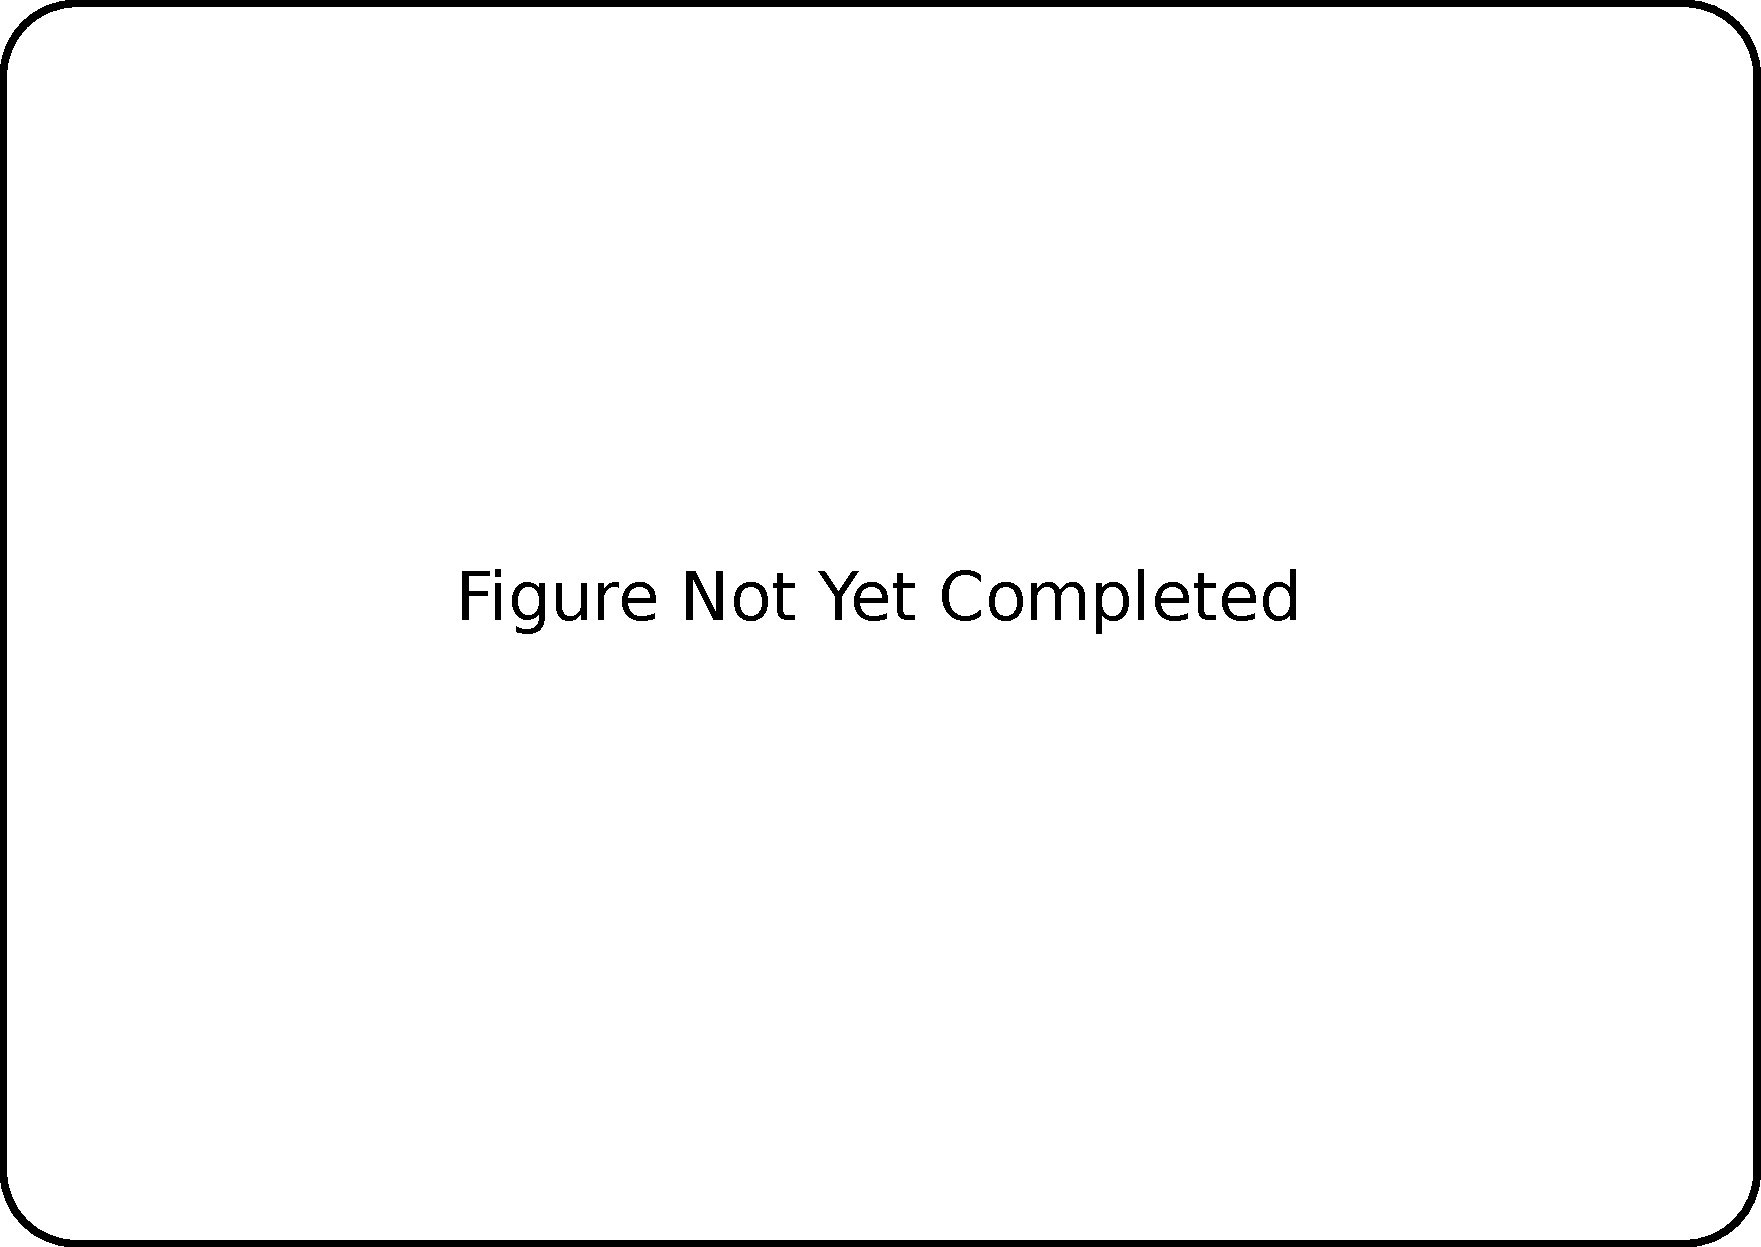
\includegraphics[width=5in]{introduction/not_finished.pdf}
%\end{center}
%\caption{Three levels of parallelism for the charge assign}
%\label{fig:pic_flowchart_parallel}
%\end{figure}

We implemented this technique in the sandbox PIC code and compared the runtime of the reduction particle-pull to the atomic particle-push. The results of this comparison can be seen in figure \ref{fig:GPUPIC_comparison}.

\begin{figure}
\begin{center}
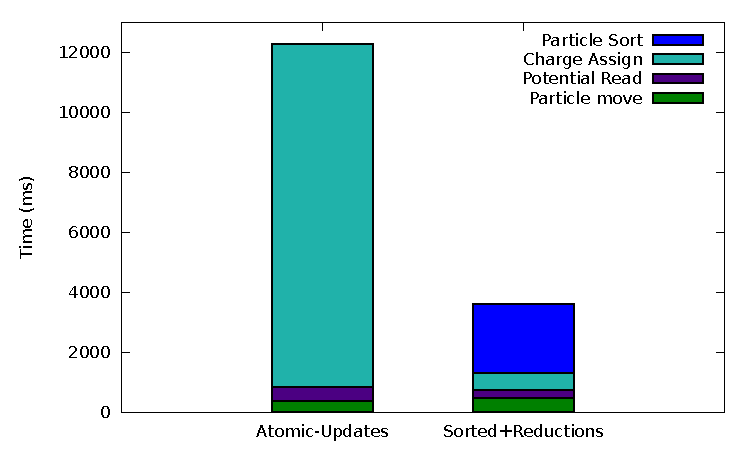
\includegraphics[width=5in]{design/atomic_vs_sorted.pdf}
\end{center}
\caption[Sandbox GPUPIC Charge Assign Comparison]{Comparison between a global atomic charge assign and a sort+reduce charge assign. Although we introduced an additional step, the total runtime is still far lower for the sort+reduce.}
\label{fig:GPUPIC_comparison}
\end{figure}




As shown in figure \ref{fig:GPUPIC_comparison}, the charge assign is on the order of 20x faster using the reduction technique, although this speed-up is somewhat offset by the sorting requirement. Sorting particles also benefits reading the potential during the advancing step. This speed-up is a result of increased cache hits due to all threads within the same thread block accessing the same addresses in the potential array. 

Although the cost of the charge assign has been reduced, an additional cost of a sorting step\footnote{It should be noted that the sort used here is an older version of the radix sort, newer versions, such as the \gls{gls:thrust} implementation are much faster} has been added. For the sandbox code, the sort step accounts for roughly 70\% of the runtime. Fortunately several other projects have figured out ways to reduce sorting costs while maintaining some of the performance gained by utilizing a sorted particle list. 

 
		\subsection{Other Codes}
It is possible to minimize the sorting requirement by expanding the sorting bins to include multiple cells, or rather, by dividing the simulation space into slabs composed of multiple cells. The advantage to this technique is that sorting is only required between slabs, not within the slabs.\cite{Abreu2011} 

This slab method, as described by Abreu et al, is used on a one thread per slab basis. One thread for each slab loops over all of the particles that belong to that slab, contributing to an array that is the same size as the slab. Once a thread completes its particle loop it writes its portion of the array to the main array, using atomic operations for guard cells.\cite{Abreu2011} Similar approaches are used by Stantchev et al and Kong et al.\cite{Stantchev2008}\cite{Kong2011}

Unfortunately it is difficult to apply the reduction version of the particle push to the slab method. The reason this is difficult is the limited \emph{\_\_shared\_\_} memory. Consider a slab with $nv_{slab}$ vertices. In order for the reduction to work we need to have $nv_{slab} \times \mathrm{nthreads}$ floats to store the results of each thread. For a typical NVIDIA GPU with 49kB \emph{\_\_shared\_\_} memory per streaming multiprocessor and 128 threads per block, we are limited to a slab of about 96 vertices per slab. This amounts to 9 cells per slab for a 3D grid, or about 3 fewer steps for a radix sort.

The approaches used by Kong and Stantchev is a hybridization of the push and pull algorithms. Here the grid is domain decomposed into sub-domains and each sub-domain assigned to a thread-block. Each thread-block has an array representing the distribution function for that sub-domain allocated in \emph{\_\_shared\_\_} memory. Particles are ordered in the particle list according to what sub-domain they reside in. Within each sub-domain the charge assign is performed like a particle push. Threads loop through a subset of the particles, check which vertices that particle is updating, and update the distribution function at those vertices. 

In order to avoid memory collisions both Kong and Stantchev use a technique similar to atomic operations. The technique that they used is called thread-tagging and is no longer needed due to the addition of atomic operations for \emph{\_\_shared\_\_} memory.\cite{Stantchev2008}\cite{Kong2011} This approach has several advantages over the reduction technique, the primary reasons being lower order sorting keys and slightly easier implementation. The disadvantage of this approach is that because it relies on atomic operations there is no guarantee that the results are deterministic since the order of the atomic operations is undefined. 







%%%%%%%%%%%%%%%%%%%%%%%%%%%%%%%%%%%%
	\section{Particle List Sort}
	\label{sec:plist_sort_design}
%%%%%%%%%%%%%%%%%%%%%%%%%%%%%%%%%%%%
		In the previous section we discussed what is required for an efficient charge assign on the GPU. In order to massively parallelize the charge assign and avoid memory collisions the particle data must be organized. Unfortunately this means introducing a new step in the PIC method, a sort step. Looking back at figure \ref{fig:GPUPIC_comparison} we can see that this sort step is now the dominant cost by a large margin\footnote{Please note that these results are for the radix sort outlined in the NVIDIA GPU computing SDK version 3.1 and provided by the CUDPP library, developed by N. Satish et al.\cite{Satish2009}}. The performance of this sort is undesirable, we would like to figure out a better way of keeping the particle data organized than the CUDPP radix sort. Fortunately this problem has been explored in great detail by nearly all past developments of GPU PIC implementations. 

Particle sorting for GPU PIC codes comes in four flavors:
\begin{itemize}
\item Partial sort using message passing. \cite{Kong2011}\cite{Decyk2011}
\item In-place particle Quicksort. \cite{Stantchev2008}
\item Linked list reordering \cite{Burau2010}
\item Full Radix Sort-by-key and reorder. \cite{Abreu2011}
\end{itemize}
Each of these methods have advantages and disadvantages. The ideal method is one that is fast for a broad range of applications and does not depend too greatly on the specifics of the problem.



	\subsection{Message Passing Sort}
	Going back to the charge assign it was concluded that sorting by cell is unnecessary. Instead the particles can be ordered according to groups of cells called bins. For most cases the dimensions of the bin will be greater than the average distance a particle will travel in a time step. There are cases in which the particle path length will be smaller than the size of a cell, however this is much more likely if the bin is several cells wide. The benefit of considering this case is that only a small fraction of the particles will leave the bin during a time step, and thus only a small number of particles need to be moved from one bin to the next. Most particles will remain in their respective bins and therefore do not need to be sorted. Instead of a full particle sort one might benefit from a method that will partially sort the particle list, only handling particles that changed bins. 

	One partial sorting method is similar to message passing. The particle list is divided into sections according to domain. Whenever a particle leaves its current bin it is flagged. Flagged particles are then moved to different sections of the particle list through a buffer. There are currently two approaches to this method. The approach taken by Kong et al, illustrated in figure \ref{fig:kong_sort} is based on integrating the buffer into the particle list. The particle list is structured such that each sub-domain's section of the particle list is divided into two regions, a data region and a buffer region. Using this particle list structure as a foundation, the sorting algorithm for a 2D mesh proceeds as follows\cite{Kong2011}:

\begin{enumerate}
\singlespace
\item Sub-domains (bins), referred to by Kong as clusters, that are adjacent horizontally are grouped into pairs called bi-clusters. This first step is odd cells on the left, even cells on the right. 
\item Particles that are moving from the left cluster to the right are copied from the left cluster into the buffer section of the right cluster. 
\item Step 2 is then repeated for particles moving from the right cluster to the left. 
\item Repeat steps 1 to 3 for bi-clusters for even cells on the left and odd cells on the right. 
\item Perform steps 1 to 4 for vertically oriented bi-clusters.  
\item For 3D repeat steps 1 to 5 for bi-clusters oriented in the third direction.
\end{enumerate}


\begin{figure}
\begin{center}
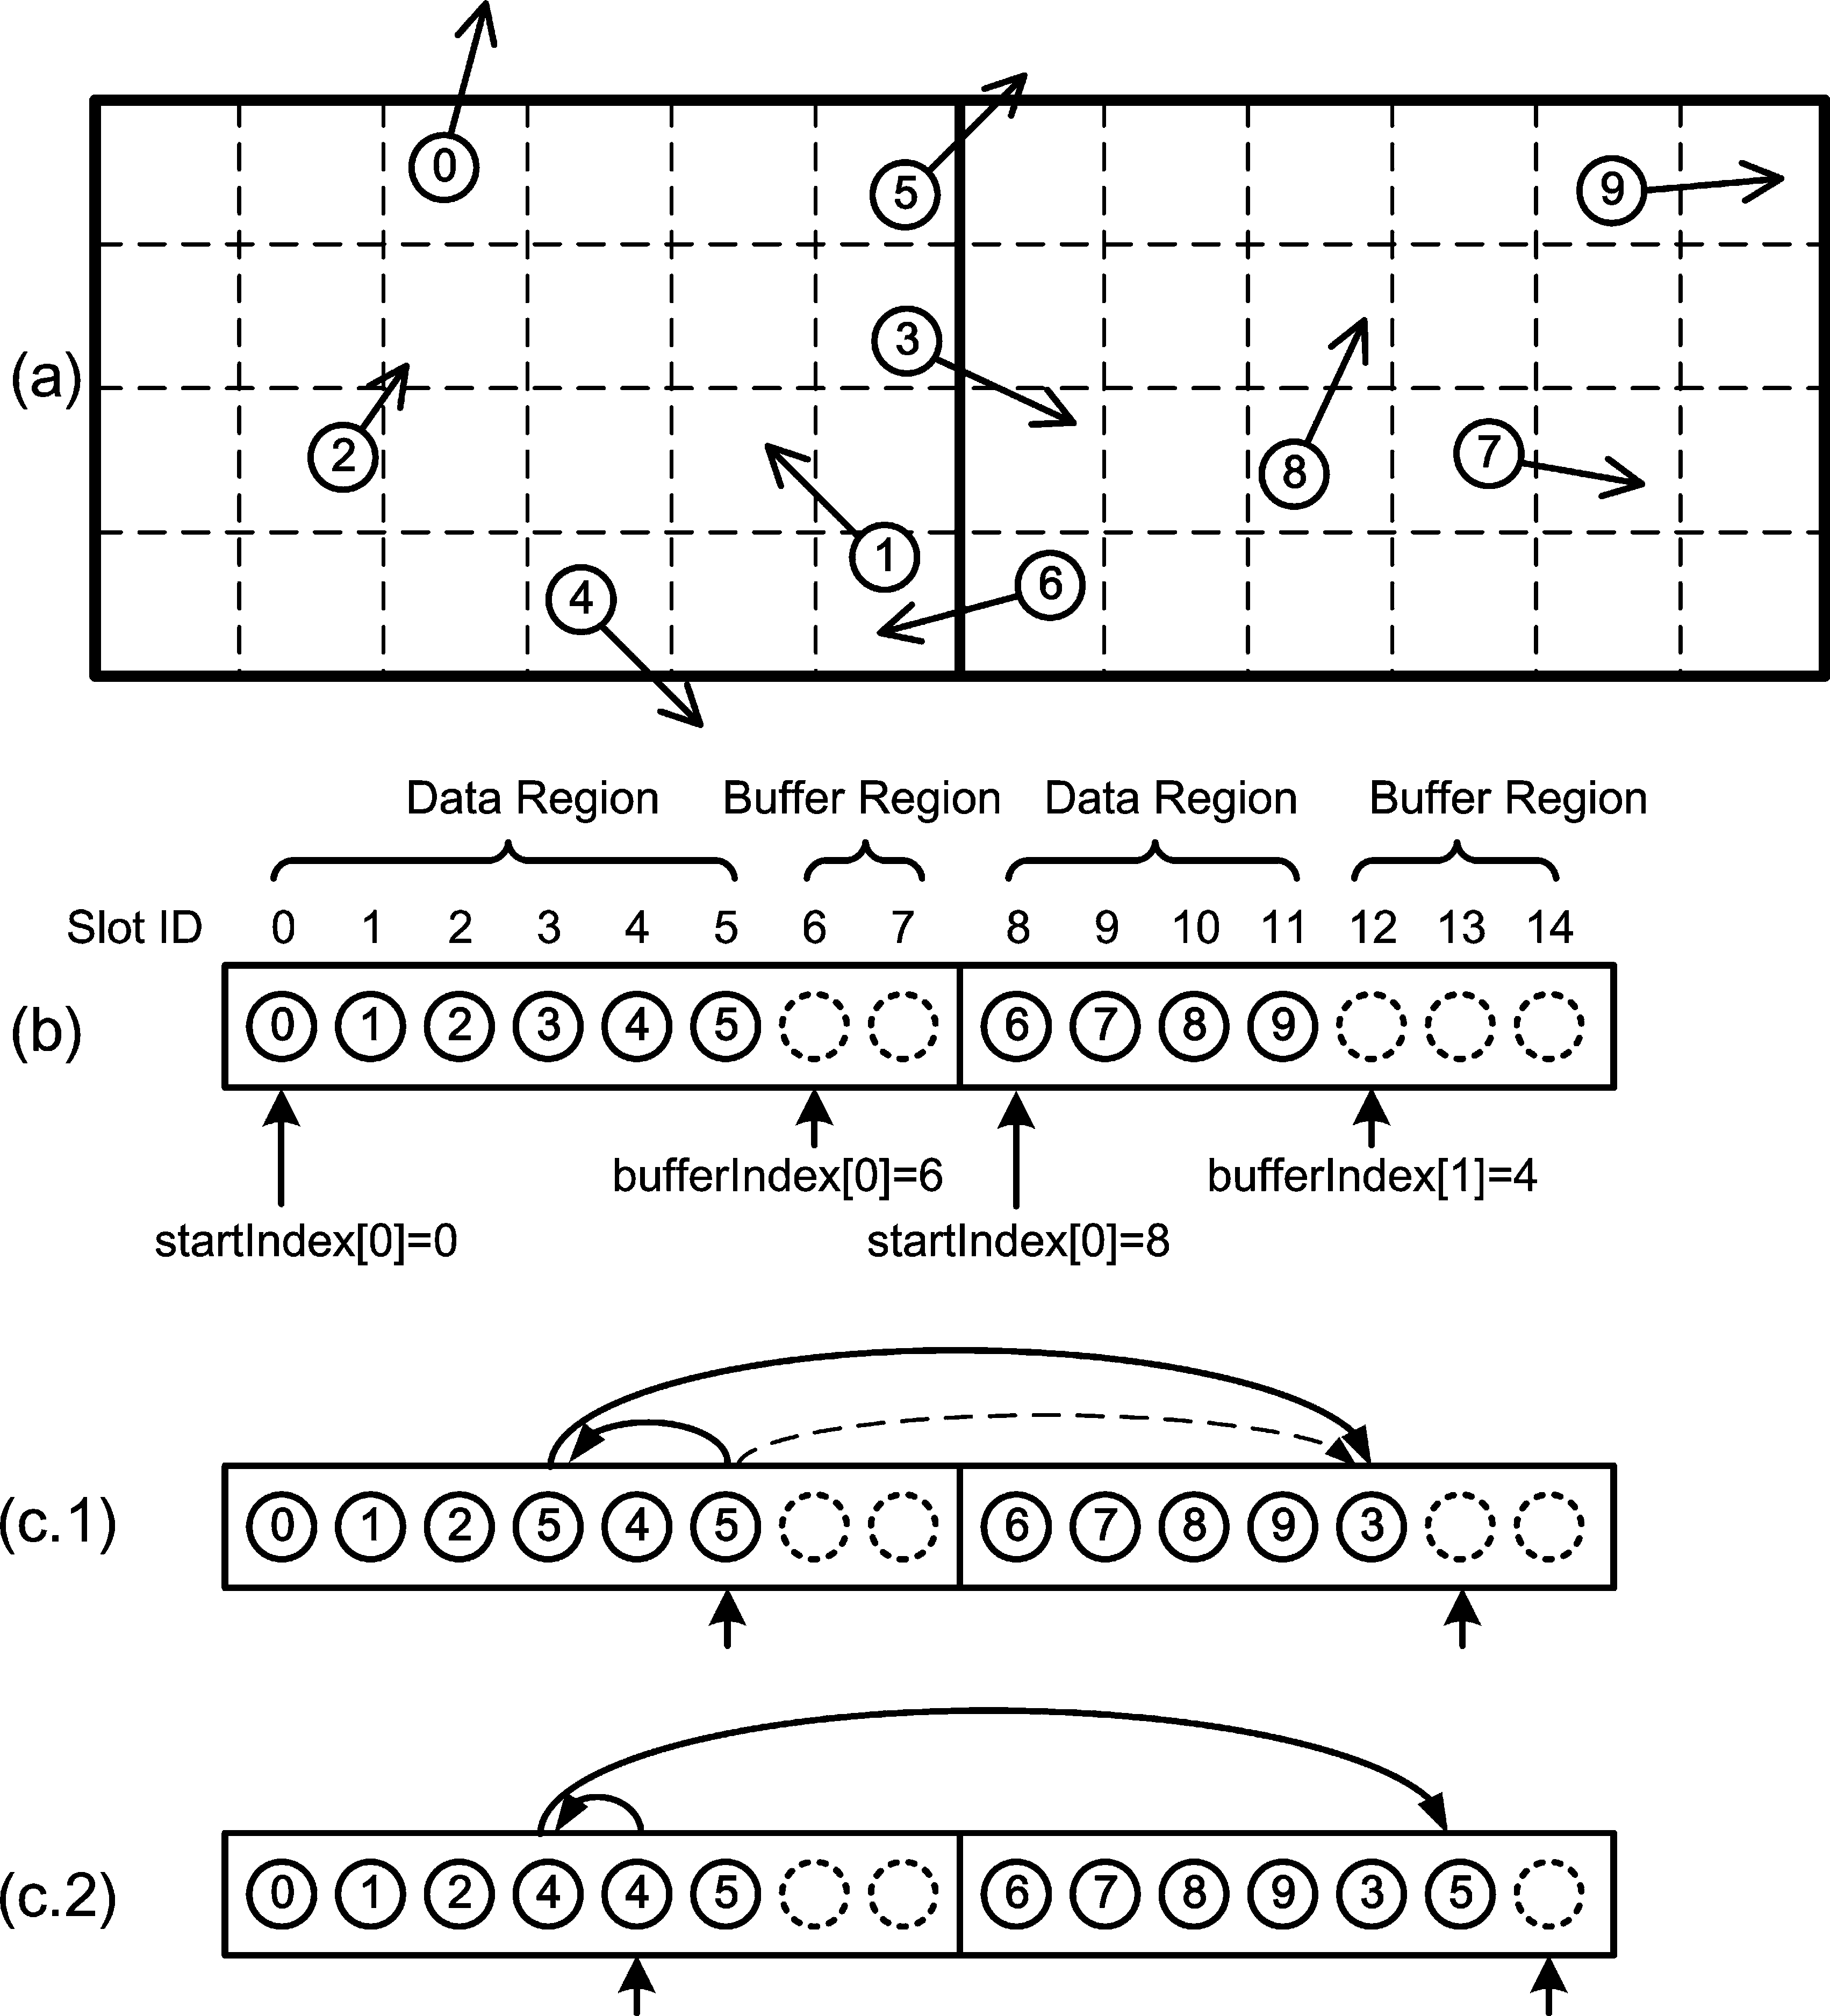
\includegraphics[width=5in]{design/kong_sort.png}
\end{center}
\caption[Message Passing Particle Sort]{Message Passing particle sort. (a) Bi-cluster of cells. (b) Data structure of the bi-cluster particle array. (c.1) Particle 3 and 5 move to the right. Particle 3 is moved first to slot 12 which frees up slot 3. Slot 3, now empty, copies the last particle in the data region, which is particle 5. Particle 5 is also moving to the right so slot 3 copies it to slot 13 and replaces the contents of slot 3 with particle 4. Image taken from \cite{Kong2011}.}
\label{fig:kong_sort}
\end{figure}

	In cases where the number of particles in a bin is greater than the number of slots in that bin, a global data reorder must be performed. This reorder is only performed when a particle to slot ratio exceeds a certain limit. When a bin exceeds this threshold the code increases the buffer for this bin by reducing the buffer of other bins. This operation is carried out through a sequence of calls to $cudaMemcpy()$ where a section of data from end of a bin is copied to the end of the buffer of the previous bin. The start index of the adjusted bin is then shifted by the amount of memory copied. \cite{Kong2011}

	This method works well if we assume that a particle will move at most one bin in any direction in a single time step. If a particle moves more than two bins, then the sort must be performed twice, one for each step that the particle moves. In the worst case scenario, where a particle can move from one bin to any other of n bins, it may take up to $n$ sort steps to put every particle in its proper bin. Another downside to this method is that it requires extra memory for the buffer. If the buffer is to small then global reorders will be performed more often. If the buffer section is too large then precious memory is wasted. 

	\subsection{In Place Particle-Quicksort}
	The second sort method, developed by George Stantchev et al, eliminates the need for a buffer array, and is applicable to cases in which particles can move any number of bins. This sort, like the message passing sort, is an ``incomplete'' which reorders only those particles that have changed bins. For this sort the particle list is divided up into ``bins" representing groups of cells to which particles in that bin belong. A separate array keeps track of the indices, called ``bookmarks" of the first and last particle of each bin. The actual sorting is based on moving particles within their respective bins and manipulating the bookmarks such that in the end all particles are where they belong. The algorithm consists of two steps, a defragmentation step and a rebracketing step. 
	
	After the particle advance some of the particles will have moved to bins with a higher bin index, and some to bins with a lower index. Since the particle list is laid out continuously in linear memory higher bins will be to the right, and lower bins to the left of the current bin. The purpose of the defragmentation step is to organize the particles within a bin into three subsets based on the direction that they are traveling, left, right, or staying. Let $P = [p_{i_1}.... p_{i_n}]$ represent a particle bin that maps to a group of cells $C$ with memory index $j$. The cell cluster that each particle resides in is denoted by $I(p)$. As shown in algorithm \ref{alg:defrag} the de-fragmentation is performed through two loops over all elements in $P$

\begin{algorithm}
	\begin{algorithmic}
		\STATE // Loop over particle bins
		\FORALL{particle bin $P_l$}
			\STATE $t_{min} \leftarrow$ lowest cell in the cluster associated with $P_l$
			\STATE $t_{max} \leftarrow$ highest cell in the cluster associated with $P_l$
			\STATE $\alpha \leftarrow$ lowest particle index of  $P_l$
			\STATE $\omega \leftarrow$ highest particle index of $P_l$
			\STATE // Forward Swapping pass 
			\FORALL{$p_i \in P_l$ in ascending order}
				\IF{$I(p_i) < t_{min}$}
					\STATE swap$(p_i, p_{\alpha})$
					\STATE $\alpha \leftarrow \alpha + 1$
				\ENDIF			
			\ENDFOR
			\STATE // Backward swapping pass
			\FORALL{$p_i \in P_l$ in descending order}
				\IF{$I(p_i) > t_{max}$}
					\STATE swap$(p_i, p_{\omega})$
					\STATE $\omega \leftarrow \omega - 1$
				\ENDIF			
			\ENDFOR
			\STATE // Now $\alpha$ and $\omega$ are the new temporary bookmarks indicating the boundaries between migrating and non-migrating particles in bin $P_l$
		\ENDFOR
	\end{algorithmic}
	\caption[Particle defragmentation]{Particle defragmentation. From Stantchev et al. \cite{Stantchev2008}}
	\label{alg:defrag}
\end{algorithm}


 Once the defragmentation step is complete the subset of the particles that are migrating must be moved to their new homes and the particle bin bookmarks updated. This step, called particle rebracketing and shown in algorithm \ref{alg:rebracket}, is performed first for all odd $l$ and then for all even $l$. Each rebracketing step starts by taking two adjacent particle bins, $P_l$ and $P_{l+1}$. Particle $p_{\omega_l}$ in bin $P_{l}$ is swapped with particle $p_{\alpha_{l+1}}$ in bin $P_{l+1}$. After the swap $\alpha_{l+1}$ is decreased by 1 and $\omega_l$ is increased by 1. This is repeated until $I(p_{\omega_l}) = I(P_l)$. The final bookmark $l$, the final particle in bin $P_l$, is given by the original values of $\alpha_{l+1}$ and $\omega_l$, $l = \alpha_{l+1}^0 - l + \omega_l^0$. The process is then repeated for all even values of $l$.

\begin{algorithm}
	\begin{algorithmic}
		\STATE // Odd Particle bins
		\FORALL{particle bin $P_l$ where $l$ is odd}
			\STATE $\alpha \leftarrow \alpha_{l+1}^0$
			\STATE $\omega \leftarrow \omega_l^0$
			\WHILE{$I(p_{\omega+1}) \ne I(P_l)$}
				\STATE swap$(p_\omega,p_\alpha)$
				\STATE $\alpha \leftarrow \alpha - 1$ 
				\STATE $\omega \leftarrow \omega + 1$ 		
			\ENDWHILE
			\STATE // Last particle $l$ in bin $P_l$ is set to:
			\STATE $l \leftarrow \alpha_{l+1}^0 - l + \omega_l^0$
		\ENDFOR
		\STATE // Repeat for even bins
	\end{algorithmic}
	\caption[Particle Re-Bracketing]{Particle ReBracketing. From Stantchev et al. \cite{Stantchev2008}}
	\label{alg:rebracket}
\end{algorithm}

	So far the method presented only works for particles moving only one bin to the left or right, but this can be expanded to include all possible magnitudes of particle movement. This is accomplished through hierarchical binning. The idea here is to create a binary tree of bins. At the first level of the tree the domain is divided into two bins, particles are sorted into the two bins using the defragmentation and rebracketing techniques described above. Once this is done each bins in the domain is cut in half and the process is repeated until the desired number of bins is reached. Traversing the entire tree takes $\mathcal{O}(N \mathrm{log} C)$ with $C$ being the total number of bins and $N$ the total number of particles. \cite{Stantchev2008}

Now when this technique is implemented in \gls{gls:CUDA} each bin is assigned to a single thread block for the defragmentation stage and two bins are assigned to each thread-block for the rebracketing stage.  Unfortunately this means that at the first level of the hierarchal binning the GPU is severely underpopulated. In cases where particle behavior is reasonably well defined we can use clever geometries for the binning tree such that the first level has multiple bins. An example of this would be dividing up a three dimensional grid into slabs and assuming that particles can only transverse one slab in a time step. One reorder pass is performed for the slab level, followed by a hierarchical method for sorting within the slab. 

This method is rather promising, it is applicable to a large variety of cases, and can be made significantly faster if assumptions about the system are integrated into the sort. A second benefit to this method is that it does not require a buffer, so more memory for particles. The downside to this algorithm is that it is very difficult to implement on the GPU and, as will be shown in figure \ref{fig:stantchev_sort_compare}, performs poorly in the general case. 


	\subsection{Linked List Ordering}
	A third method of maintaining particle order, used by Heiko Burau et al is based on never moving the particle data from its original position in memory. Instead, each cell contains a pointer to the last particle in its local linked list, and each particle contains a pointer to its predecessor in its cell's linked list. When a particle changes cells it is deleted from the old cell's linked list and appended to the new cell's linked list. Particle list insertions and deletions are handled by atomic memory operations. \cite{Burau2010}

	There is one major issue with this approach, namely, the reordered access pattern can severely reduce performance due to un-coalesced memory accesses. Burau notes that this does in fact occur with the current deposition routine being the most affected routine. \cite{Burau2010} %Unfortunately it is difficult to perform a meaningful comparison between this approach and other approaches with the information in the paper ``PIConGPU: A Fully Relativistic Particle-in-Cell Code for a GPU Cluster".

	\subsection{Full Sort using Sort from the THRUST Library}
	The final and most general option is performing a full sort using the radix sort provided with the \gls{gls:thrust} library.\cite{NVIDIACorporation2011a} The organization of the particle list is similar to the message passing and QuickSort methods, that is, particles are grouped into bins that represent clusters of cells. Particles are sorted by populating an array containing the bin indices of all of the particles along with an array containing the indices of all the particles in the particle list. The binID / particleID arrays are used in the \gls{gls:thrust} sort\_by\_key$()$ function. Once the particle indices have been sorted, a kernel is launched in which each thread reads in a particle ID and then uses that ID to copy particle data from the original list into the new sorted list. 

	With the newer versions of the \gls{gls:thrust} sort this method can be very fast, as well as simple to implement. This method is also very general and applicable to all PIC codes as it is completely independent of the physics of the problem at hand. On the other hand, the generality of this method can be a down side as there is no way to improve this routine based on the physics of the system. The message passing sort and QuickSort methods can perform better than the full sort in cases where the maximum distance that particles will travel in a given time step is known to be small. In this case, the message passing sort and QuickSort methods will take fewer iterations, and therefore perform better. In cases where particle movement is completely undefined the \gls{gls:thrust} sort wins. A comparison of the \gls{gls:thrust} sort and the Stantchev sort can be seen in figure \ref{fig:stantchev_sort_compare}. 





\begin{figure}
\begin{center}
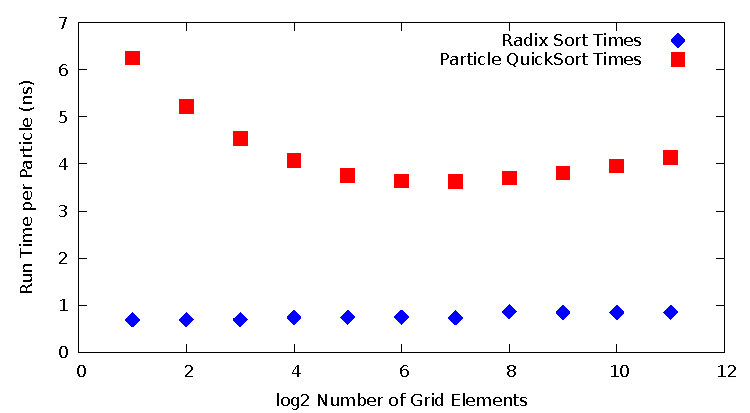
\includegraphics[width=5in]{design/sort_compare.pdf}
\end{center}
\caption[Comparison of Particle QuickSort and the \gls{gls:thrust} radix sort.]{Comparison of Particle QuickSort and the \gls{gls:thrust} radix sort. The latest implementation of the THRUST radix sort is very fast for a generalized problem. However, the Particle QuickSort can perform significantly better if constraints on particle movement are }
\label{fig:stantchev_sort_compare}
\end{figure}

The data shown in figure \ref{fig:stantchev_sort_compare} was generated using a simple code that populates a partially ordered particle list and then sorts this list. The amount of data for each particle is similar to that of SCEPTIC3D, six floats for position and velocity, and one integer to keep track of bin index. The ``grid" is represented by a series of bins, there is no need to represent individual cells for this comparison. The partial ordering is achieved by looping over the particle list and assigning each particle $p_i$ to bin $\mathrm{floor}(\frac{N_{part}}{G} i)$. Where $N_{part}$ is the total number of particles, $G$ is the size of the grid, and $i$ is the particle index. The ``partial" part of the ordering is achieved by drawing a random number for each particle, if this number is less than $R$, then a second random number is drawn to determine if the particle is being placed in the previous or next bin. The boundary conditions are periodic such that particles in bin 0 that are being placed in a lower bin end up in bin $G-1$ and particle in bin $G-1$ that are being shifted up will end up in bin 0. The number $R$ can be adjusted in order to adjust the fraction of particles that are moving. For the data shown in figure \ref{fig:stantchev_sort_compare} $R = 0.2$, $N_{part} = 2^{24}$, and G ranges from $2^1$ to $2^{12}$. 

Overall the thurst sort has the benefits of being easy to implement, very general, and is part of an externally maintained library that will be updated as GPU hardware changes. Fortunately the \gls{gls:thrust} sort is also much faster than the CUDPP radix sort. The performance of the \gls{gls:thrust} sort is fast enough that it is no longer the dominant cost. The downside to this sort is that it also requires allocation of buffer memory. The amount of memory required for this buffer array can be reduced by using separate arrays for each element of the particle list, which will be discussed in detail in the next section. For now the \gls{gls:thrust} sort is simple, fast, and will therefore be the method used in the final implementation. 

\subsection{Spatial Indexing}

One way that sort performance can be improved is through use of space filling curves, such as a Z-order curve for cell-cluster indexing. Utilizing a space filling curve for the cluster indexing preserves the spatial ordering of the clusters in their layout in memory. This aids the sort by reducing the distance that particles must move in memory whenever they change clusters. We will use a z-order curve to index the cell clusters, since it is fairly simple to implement.

%%%%%%%%%%%%%%%%%%%%%%%%%%%%%%%%%%%%
	\section{Particle List Structure}
%%%%%%%%%%%%%%%%%%%%%%%%%%%%%%%%%%%%

Another major design question is the choice of data structure for the particle list. In the serial version of SCEPTIC3D the particle data is laid out in a 6xN array of reals in fortran. In C this layout corresponds to an array of six element structures. The array of structures format performs well on the CPU since only one particle is being operated on at a time, this means that data from only a single particle will be required at a given time. On the GPU things are different. Whenever data accesses are performed on the GPU a group of 32 threads, a warp, executes memory requests for the same element, but from 32 different particles. If these addresses are not sequential then the request will be divided up into as many 128 byte cache-line transactions as it takes to fulfill the requests from all 32 threads. In kernels where all six elements will be used soon after one another, such as in the move kernel, this is not a big issue. When the request for the first element is read from global memory, the data for the other 5 elements will also be retrieved from global memory. For the most part cache hits are almost as fast as registers, so subsequent requests for the other 5 elements will result in fast cache hits. Unfortunately this is not true of kernels in which only a subset of the elements is required, such as when calculating the particle bin index of each particle relies only on the particle's position. \cite{NVIDIACorporation2011}

\begin{figure}
\begin{lstlisting}[frame=single]
class XPchunk // Array of Structures
{
public:
	float x,y,z,vx,vy,vz;
};

class XParray // Structure of Arrays
{
public:
	float* x,y,z,vx,vy,vz;
};
\end{lstlisting}
\caption{Array of Structures and Structure of Arrays}
\end{figure}   
	
	The alternative is to use a structure of arrays, which corresponds to the transpose of the particle list structure in the fortran code. The main benefit of a structure of arrays is that reading in a single element of the particle list for 32 particles corresponds to a 128 byte transfer, the size of the cache line transaction. None of the bandwidth is wasted. This only takes 6 reads to global memory, no reads to cache. Reading in the elements of the array of structures results in at least 6 reads to global memory for the first element, followed by 5 reads from cache in the best case scenario. In order to test this the sandbox GPU PIC code was run with both an array of structures (AoS) and a structure of arrays (SoA). The results of this test are shown in figure \ref{fig:struct_compare}. 
	
\begin{figure}[h]
\begin{center}
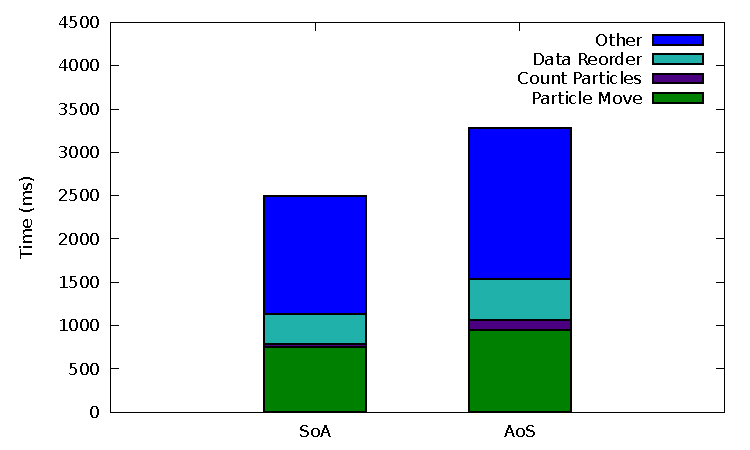
\includegraphics[width=5in]{design/soa_vs_aos.pdf}
\end{center}
\caption[Particle List Structure Comparison]{Execution times of main steps for Array of Structures and Structure of Arrays. Count Particles and Data Reorder are steps used for a sorted particle list. Count Particles counts the number of particles in each sub-domain. Data Reorder reorders the particle list data after the binindex / particle ID pair have been sorted by the radix sort.}
\label{fig:struct_compare} 
\end{figure}



The most substantial benefit to using the the structure of arrays is the smaller buffer required for the particle sort. Using a structure of arrays we only need a 1xN array of floats to sort each element of the particle list into. We would need a 6xN floats for sorting the array of structures. This approach scales well with more complicated particles that must store more information. For SCEPTIC3D we have a total of 6 floats for spatial and velocity components, one 32-bit integer for the particle index, one float to store previous time step for reinjections, and a 16-bit integer for the binID. Using a structure of arrays the memory requirements imposed by the sorting step only increase the memory required per particle by 12\%. The standalone buffer array can also be useful for other uses, such as stream compactions and reductions of diagnostic outputs. 

The main downside of the structure of arrays is that a transpose is required for particle data transfers between the fortran SCEPTIC3D code and the GPU code. Performing this transpose on the GPU would require a large amount of memory, which would reduce the total number of particles that could be run. Performing it on the CPU is more costly computationally, but saving GPU memory provides better performance overall.  




%%%%%%%%%%%%%%%%%%%%%%%%%%%%%%%%%%%%
	\section{Particle Advancing}
%%%%%%%%%%%%%%%%%%%%%%%%%%%%%%%%%%%%
	Implementing SCEPTIC3D's particle advance on the GPU is fairly straightforward, and is nearly identical to the CPU implementation. The primary design challenge here is dealing with reinjections.

The SCEPTIC3D particle advance algorithm is as follows:

\begin{algorithm}
	\begin{algorithmic}
		\FORALL{$p_i \in$ particles}
		\STATE $p_i \leftarrow \mathrm{move}(p_i,\Delta t)$
		\WHILE{$p_i\rightarrow \mathbf{x} \notin \mathrm{Domain}$}
			\STATE $\Delta t_{prev} \leftarrow \Delta t - \frac{\|\mathbf{\mathrm{exit}} - \mathbf{x}_i^0\|}{\|\mathbf{v}_i\|}$
			\STATE $p_i \leftarrow \mathrm{Reinject}()$
			\STATE $p_i \leftarrow \mathrm{move}(p_i,\Delta t_{prev})$
		\ENDWHILE	
		\ENDFOR
	\end{algorithmic}
	\caption{SCEPTIC3D Particle Advancing}
	\label{alg:padvnc}
\end{algorithm}

Reinjections on the CPU are performed whenever a particle leaves the computational domain. When this event occurs, the code first determines the exact point during the timestep that the particle left the grid. A new particle is reinjected by calculating a new position and velocity as described by Patacchini \cite{Patacchini2007} and advanced the remainder of the times step. Additional reinjections are performed if the new particles also leaves the domain. 

Unfortunately this method does not work well on the GPU. If this same algorithm were to be used on the GPU it would result in a large amount of execution divergence within a warp, which serializes the execution of the warp. Calculating new random positions and velocities is also expensive. Ideally all of the particles will be advanced, then only the subset of particles being reinjected will be operated on. In \gls{gls:CUDA} this is done by compacting the particle stream to a list that contains only particles undergoing reinjection. This list is repopulated with new positions and velocities drawn from a pool of precalculate values on the host. This compacted particle list is still a particle list, and can be advanced by recursively calling algorithm \ref{alg:padvnc}. Once the reinjection list has been advanced the code returns to the advancing method for the main list. Further details concerning the implementation of this method will be presented in section \ref{sec:handling_reinjections}.






%% This is an example first chapter.  You should put chapter/appendix that you
%% write into a separate file, and add a line \include{yourfilename} to
%% main.tex, where `yourfilename.tex' is the name of the chapter/appendix file.
%% You can process specific files by typing their names in at the 
%% \files=
%% prompt when you run the file main.tex through LaTeX.
\chapter{Implementation}

	\section{Constraining Grid Dimensions}
		\subsection{Constraints}
There are two constraints that the grid dimensions must conform to. The first is set by the requirements of a simple z-order curve, the second is set by the size of the on chip shared memory. These constraints are expressed mathematically through the grid dimensions, $n_r, n_{\theta}, n_{\psi}$, and the block subdomain dimensions, $nb_r, nb_{\theta}, nb_{\psi}$.
		
\begin{equation}
\frac{n_r}{nb_r} = \frac{n_{\theta}}{nb_{\theta}} = \frac{n_{\psi}}{nb_{\psi}} = n_{virtual}
\end{equation} 

Where $n_{virtual}$ is the number of blocks that the grid is divided into in any dimension. In order to fully satisfy the constraints for a simple z-order curve, $n_{virtual}$ must be a power of 2.

The second constraint on the grid dimensions is set by the hardware. The goal is to maximize the shared-multiprocessor occupancy for the chargeassign stage of the code. Given that each block has the maximum number of threads, 512, and each thread requires roughly 25 registers, then the maximum number of threadblocks that can exist simultaneously on a single SM is 2. This means that each block can be allocated half of the total amount of shared memory on the SM. Compute capability 2.0 GPUs have 49152 bytes of shared memory per SM. Running two blocks per SM provides each block with 24576 bytes of shared memory each, or 6144 floats per block. The maximum that all three block dimensions can be is 18. For the sake of simplicity this sets $nb_r, nb_{\theta}$, and $nb_{\psi} \le 18$. 

A third, loose constraint can be set in order to force a minimum nuber of threadblocks for the charge-assign. The command line option ``--minbins\#'' sets the parameter $n_{virtual} = \#$. This is useful in ensuring that enough threadblocks are launched to populate all of the SMs on the GPU. To populate all of the SMs on a GTX 470 the code would need to launch at least 28 thread-blocks. For a GTX 580 with 16 SMs 32 thread-blocks are required to fill all of the processors.  
		\subsection{Holding to the constraints}

	\section{Particle List Transpose}
As previously mentioned the particle list structure on the GPU is different than the structure on the CPU. On the GPU particles are stored in a structure of arrays, while on the CPU they are stored in a 6x$n$ array. This means that in order to copy a particle list generated on the CPU to the GPU, or vice versa, the particle list must be transposed. The two main places in the code where this matters is when the particle list is initially populated at the start of the code, and when copying a list of pre-calculated reinjection particles from the CPU to the GPU at every time step during the advancing phase.

The particle list transpose was implemented on the CPU in two different ways depending on the compiler used and the available libraries. A GPU based particle list transpose is significantly faster than a CPU based transpose. However, the GPU has a very limited amount of DRAM compared to the CPU, and it is preferable to use as much of the available GPU memory as possible for the main particle list. In any case transposing the entire particle list only occurs once, but a smaller transpose is performed every time step for reinjected particles. This means that while a faster transpose is preferable, it represents so little of the total computation time that it is not worth developing a complicated in place GPU transpose.  

	\section{Charge Assign}
	As previously mentioned, the charge assign is one of the most difficult funcitons to parallize. The niave approach of applying a thread to every particle and atomically adding each particles contribution to an array in global memory is very slow. Grouping the particles spatially allows the majority of the atomic operations to be done in the context of shared memory which is much faster than global memory. The resulting algorithm resembles basic domain decompositon where each thread-block represents a seperate sub-domain. The actual charge deposition method in this shceme is very similar to the niave approach, with a key difference being that all the threads in the thread block are operating on shared memory. Once all particles in the subdomain have contributed to grid in shared memory it takes only a small number of global memory accesses to write the contributions of a large number of particles to the main array. 

	\subsection{Domain Decomposition}

	\subsection{Particle Bins}
	\subsection{Particle Push}
		- Atomic writes to shared memory
		- Block atomic writes to global memory

	\section{Particle List Sort}


	\section{Poisson Solve}

	\section{Particle List Advance}

		\subsection{Checking Domain Boundaries}
		\subsection{Diagnostic Outputs}
		\subsection{Handling Reinjections}






\chapter{Performance}
\label{ch:performance} 
	Unless otherwise specified the following tests were performed using two CPU cores or two GPUs, with \gls{ac:mpi} as the interface between multiple threads. The machine specifications for system 1 are as follows:
\begin{itemize}
	\item CPU: Intel Core i7 930 @ 2.8GHz.
	\item Memory: 12GB (3 x 4GB) DDR3 - 1333MHz ECC Unbuffered Server memory. 
	\item GPUs: 2x EVGA GeForce GTX 470 1280MB, 607 MHz / 1215 MHz, Graphics / Processor Clock. 
	\item Motherboard: ASUS P6T7 WS Supercomputer Intel x58.
\end{itemize}
%	\section{Test Setup}
%		\subsection{Parameter Space Explored}
%		\subsection{Machine Parameters}
%		\subsection{Memory Bandwidth Comparison}

Typical total\footnote[1]{Total run time includes \gls{ac:mpi} reduces and various other subroutines that were not ported to the GPU} speedups on this setup are on the order of 40x. A detailed breakdown of the run times per particle per time step and the speedup achieved by the GPU code. These runs were performed on 2 GPUs with 17 million particles per GPU and a grid size of $64^3$ using two different GPUs and CPUs. The first setup has already been mentioned and the second setup, system 2, is comprised of 2x  Intel(R) Xeon(R) CPU E5420 @ 2.50GHz and 1x NVIDIA GeForce GTX 590. The GTX 590 is a double GPU card with 2 x 512 processing cores clocked at 630 MHz, and 2x 1.5 GB ram. Figures \ref{fig:speedup} and \ref{fig:speedup2} show the run times and speedups for the CPU and GPU on both of these systems. It is important to note that system 2 has a slower processor and lower memory bandwidth than system 1. The lower CPU performance combined with a faster GPU gives system 2 much higher speedup values compared to system 1.

\noindent \begin{figure}
\begin{center}
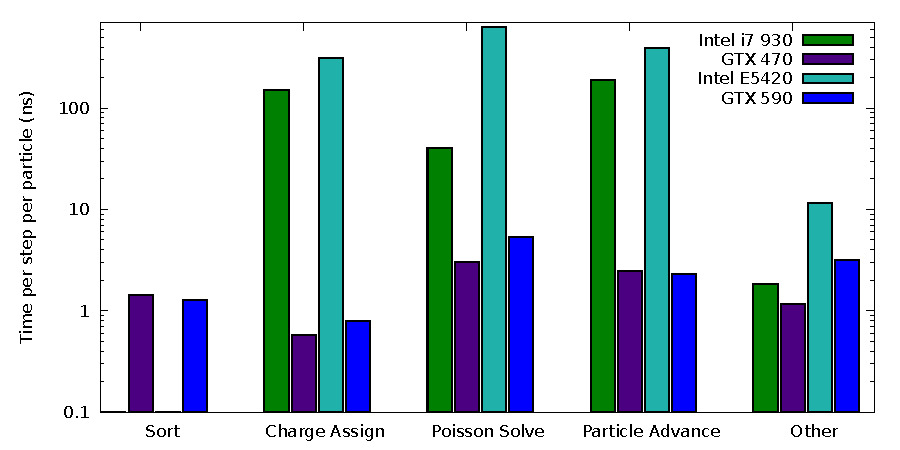
\includegraphics[width=6in]{performance/architecture_compare.pdf}
\end{center}
\caption[CPU and GPU Runtime comparison]{CPU and GPU Runtime comparison for a GTX 590 vs an Intel(R) Xeon(R) CPU E5420. Test was performed using 2 \gls{ac:mpi} threads handling 42 million particles each on a $64^3$ grid.}
\label{fig:speedup} 
\end{figure} 

\noindent \begin{figure}
\begin{center}
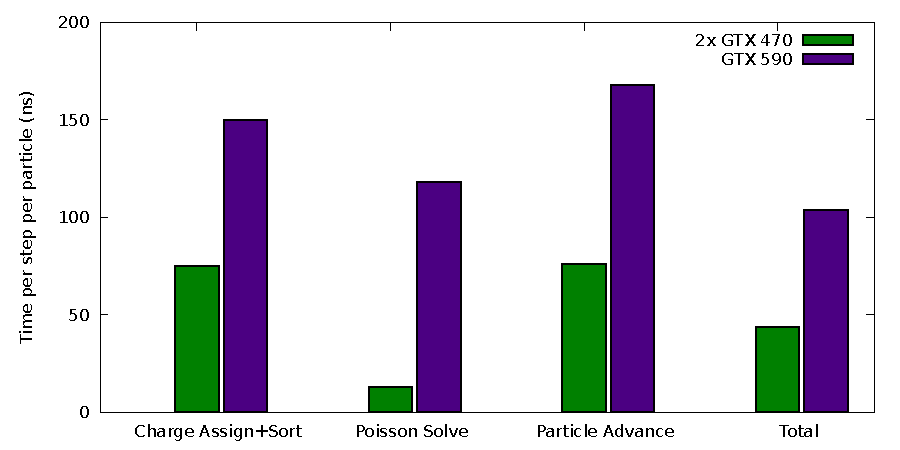
\includegraphics[width=6in]{performance/architecture_speedup_compare.pdf}
\end{center}
\caption[CPU and GPU Speedup comparison]{CPU and GPU Speedup comparison for a GTX 590 vs an Intel(R) Xeon(R) CPU E5420. Test was performed using 2 \gls{ac:mpi} threads handling 42 million particles each on a $64^3$ grid. The difference in results is due primarily to the different hardware present on the two systems. The system with the GTX 590 is older than that used with the 2x GTX 470's}
\label{fig:speedup2} 
\end{figure} 



The initial results indicate that a very high speedup was achieved for the charge assign and particle advance routines. It should also be noted that ordering the particle data allows for an incredibly fast charge assign. After accounting for the time that it takes to sort the particle list, the speedup is a more modest 75x. In other codes the primary concern has been how to quickly and efficiently keep the particle list sorted. The results in figure \ref{fig:speedup} indicate, that with the latest \gls{gls:thrust} sort, speeding up the particle list sort is no longer a major issue. The sort step could be improved by taking into account problem specific properties of a given pic code, but considering the ease of use and generality of the \gls{gls:thrust} sort, it is unlikely that developing an optimized problem-specific sorting routine would really be worth it. 



	
	\section{Particle list size scan}
The following tests were performed to explore the dependence of SCEPTIC3DGPU's runtime on the total number of particles in the simulation for two standard grid sizes. Figure \ref{fig:nptclsize_scan128x64x64} was performed on a 128x64x64 grid, and figure \ref{fig:nptclsize_scan64x32x32} was performed on a 64x32x32 grid. Since the run times for the GPU and the CPU vary by such a large degree, a comparison between the two architectures is represented by the speedup factor, $\tau_{\mathrm{cpu}}/\tau_{\mathrm{gpu}}$. The speedup factor as a function of the total number of particles is shown in \ref{fig:nptclsize_scan_speedup}.

\begin{figure}
\begin{center}
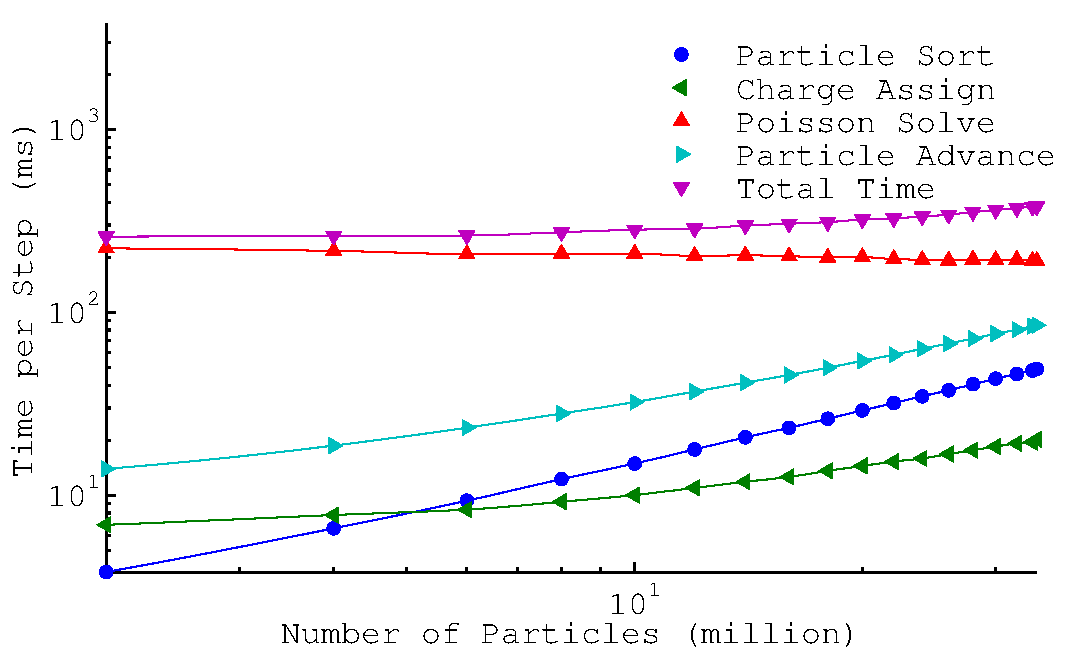
\includegraphics[width=6in]{performance/nptclsize_scan128x64x64ons8bins.pdf}
\end{center}
\caption[Number of Particles Scan on a 128x64x64 grid]{Number of Particles Scan on a 128x64x64 grid. Far more particles are needed in order to prevent the Poisson solve from being the dominant cost.}
\label{fig:nptclsize_scan128x64x64}
\end{figure}

\begin{figure}
\begin{center}
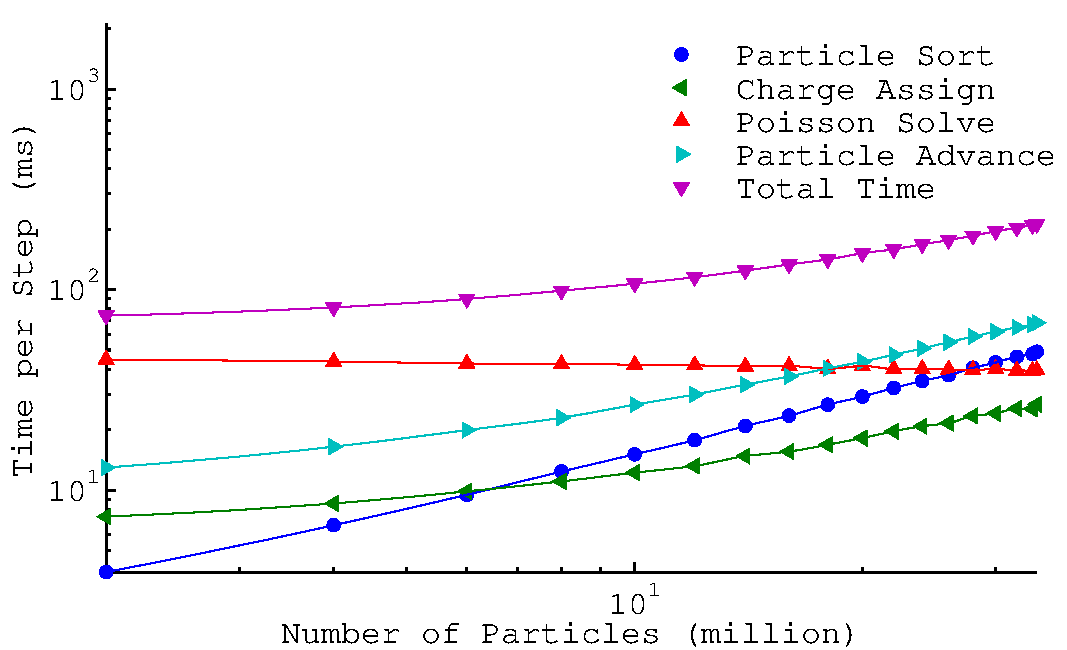
\includegraphics[width=6in]{performance/nptclsize_scan64x32x32ons8bins.pdf}
\end{center}
\caption[Number of Particles Scan on a 64x32x32 grid]{Number of Particles Scan on a 64x32x32 grid. At about 20 million particles, the particle moving steps become the dominant costs.}
\label{fig:nptclsize_scan64x32x32}
\end{figure}

\begin{figure}
\begin{center}
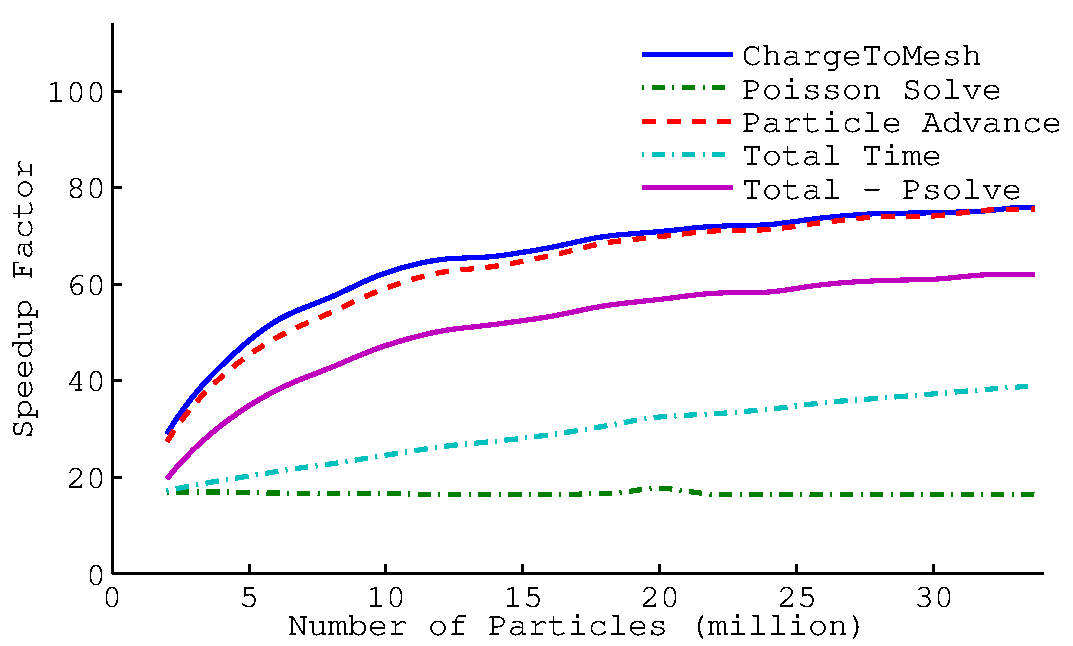
\includegraphics[width=6in]{performance/nptclspeedup_scan128x64x64ons8bins.pdf}
\end{center}
\caption[Speedup factor Number of Particles Scan on a 128x64x64 grid]{Speedup factor Number of Particles Scan on a 128x64x64 grid. The speedup factors for both the charge assign and particle advance are very similar, and follow similar trends. The total speedup is greatly reduced in this case because of the relatively high cost of the Poisson solve.}
\label{fig:nptclsize_scan_speedup}
\end{figure}

In the case of the 128x64x64 grid the Poisson solve is by far the most expensive computation for all ranges of particles. For a smaller grid, 64x32x32, the Poisson solve dominates for fewer than 15 million particles, but drops below the particle advance and particle sort for more than 15 million particles. Perhaps the most interesting behavior is best observed in the speedup factor, figure \ref{fig:nptclsize_scan_speedup}, which shows a very steep rise in the speedup factor below 10 million particles. This behavior indicates that anything fewer than 10 million particles will not saturate the gpu. This behavior can also be seen in the figures \ref{fig:nptclsize_scan128x64x64} and \ref{fig:nptclsize_scan64x32x32} by the fact that the particle advance, charge assign, and total time converge to linear behavior at large numbers of particles. 

A second interesting characteristic is the fact that the speedup factor curves do not fully flatten out between 10 million particles and 30 million particles. This is due in part to some small cpu costs within these routines, namely host-device transfers of data that does not scale with the number of particles. For the GTX 470 with 1280 MB of memory 17 million particles is about the limit for a single gpu. Looking at figure \ref{fig:nptclsize_scan_speedup} it is not unreasonable to conclude that with an even larger performance boost can be attained simply by increasing the amount of available device memory.

	
\section{Grid Size scan}
So far the results indicate that the GPU is very good at moving the particles and writing the density array. In fact the GPU is so good at this that it is wasteful to not run as many particles on the gpu as physically possible. This brings us to the second main parameter of interest, the grid size. Generally speaking we would expect to see three of the subroutines display scaling with gridsize, but through different mechanisms. The Poisson solve should scale roughly linearly with the number of grid elements, while more subtle scalings are dominant for the charge assign and particle advancing routines. 

	\subsection{Absolute Size}
	In order to get a reasonable idea of how SCEPTIC3DGPU scales with grid size three sweeps of the grid size parameter were performed using 8, 16, and 34 million particles. There are two separate plots for each particle number due to the fact that for large grid sizes the number of bins must be increased in order to account for shared memory size restrictions. Since some of the scalings for the particle advance and charge exchange depend primarily on the number of elements per bin and not the absolute grid size plotting the results for $8^3$ bins and $16^3$ bins would be misleading.

The primary routine of interest here is the Poisson solve, which takes roughly $\sqrt[3]{G}$ iterations of operations that are roughly $\mathcal{O}(G)$, where G is the total number of grid elements. This scaling can be seen clearly in figures \ref{fig:grid_scan16ptcls8bins} through \ref{fig:grid_scan34ptcls16bins}. However, much like the number of particles scaling of the particle advance and charge assign, there is a region in which the GPU Poisson solver is not saturated and beats the normal scaling. Once the GPU is saturated the Poisson solve behaves as expected, scaling roughly linearly with the total number of grid elements. 

%\begin{figure}[H]
%\begin{center}
%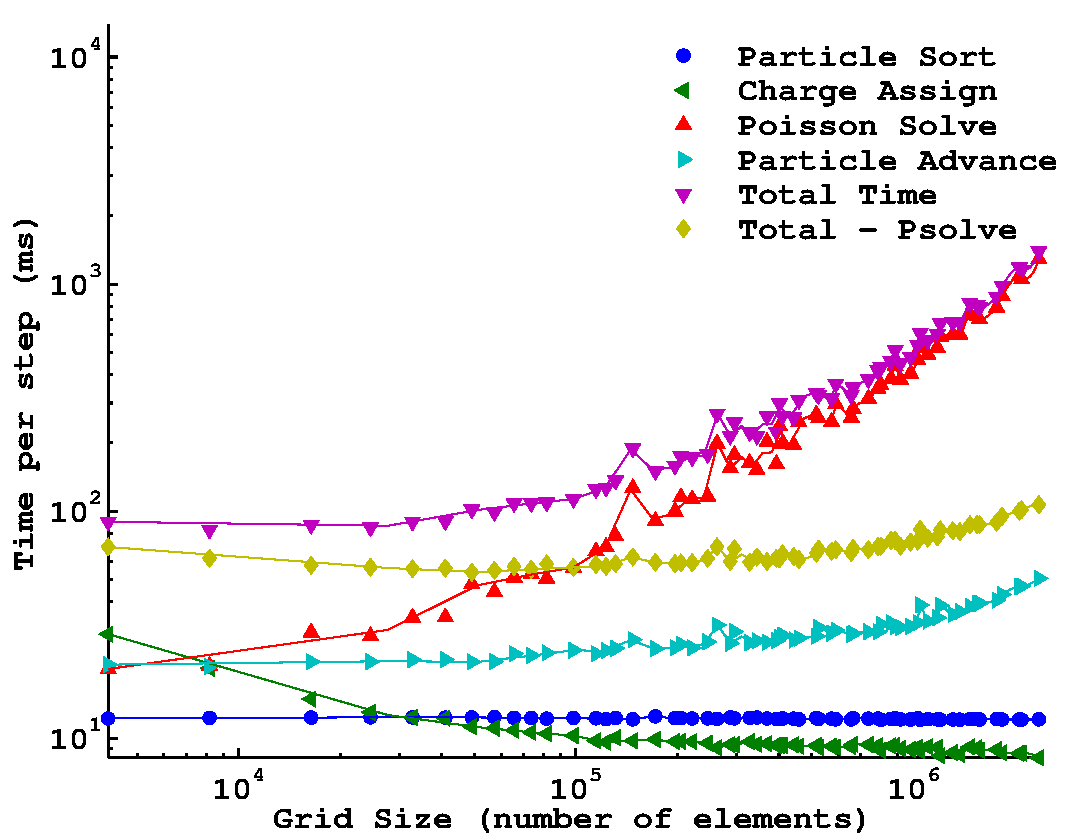
\includegraphics[width=6in]{performance/gridsize_scan8ptcls8bins.pdf}
%\end{center}
%\caption{Gridsize Scan with 8 million ptcls, and $8^3$ bins}
%\label{fig:grid_scan8ptcls8bins}
%\end{figure}


%\begin{figure}[H]
%\begin{center}
%
\includegraphics[width=6in]{performance/gridsize_scan8ptcls16bins.pdf}
%\end{center}
%\caption{Gridsize Scan with 8 million ptcls, and $16^3$ bins}
%\label{fig:grid_scan8ptcls16bins}
%\end{figure}


\begin{figure}
\begin{center}
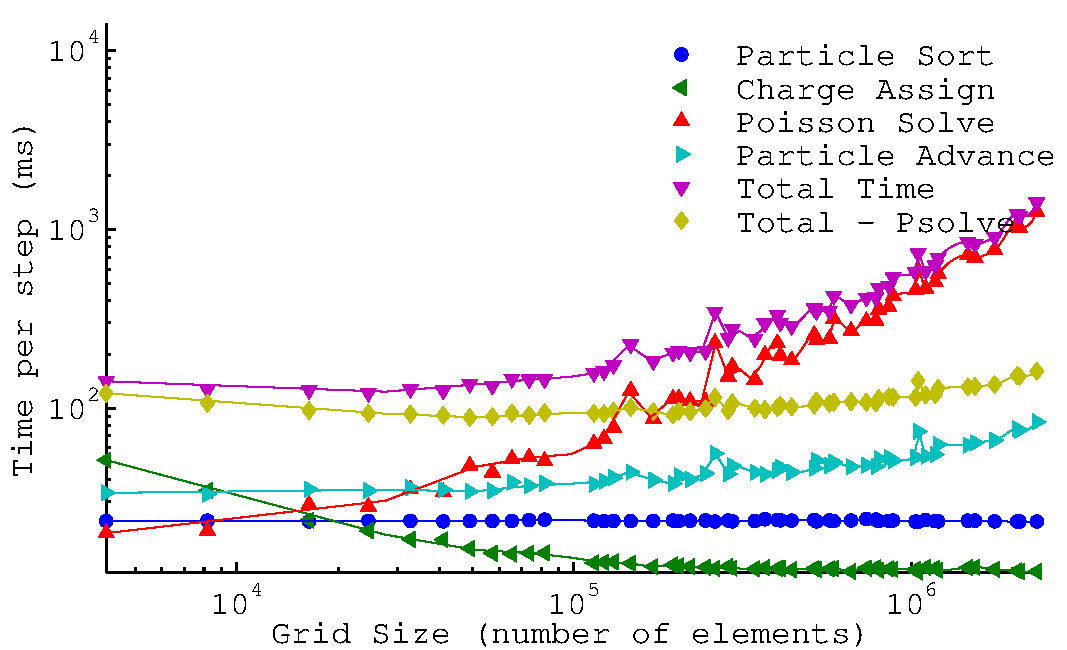
\includegraphics[width=6in]{performance/gridsize_scan16ptcls8bins.pdf}
\end{center}
\caption[Gridsize Scan with 16 million particles and $8^3$ bins]{Gridsize Scan with 16 million particles, and $8^3$ bins}
\label{fig:grid_scan16ptcls8bins}
\end{figure}

\begin{figure}
\begin{center}
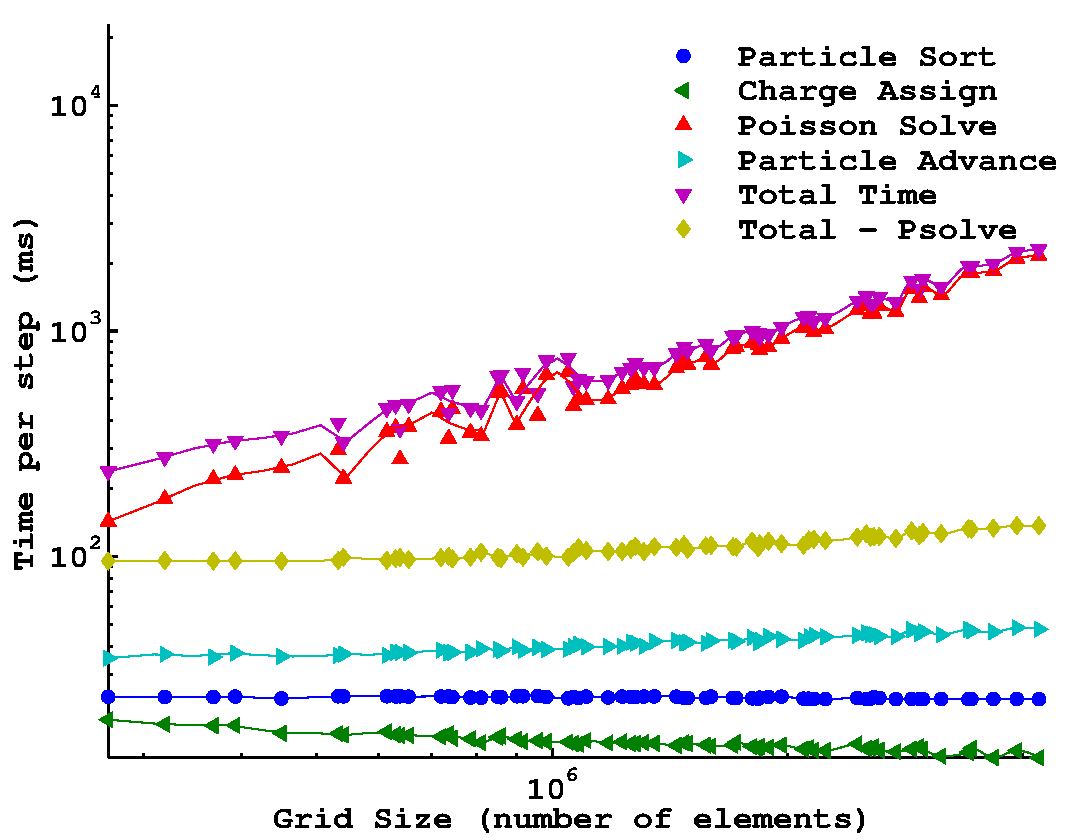
\includegraphics[width=6in]{performance/gridsize_scan16ptcls16bins.pdf}
\end{center}
\caption[Gridsize Scan with 16 million particles and $16^3$ bins]{Gridsize Scan with 16 million particles, and $16^3$ bins. The total runtime is entirely dominated by the Poisson solve.}
\label{fig:grid_scan16ptcls16bins}
\end{figure}

\begin{figure}
\begin{center}
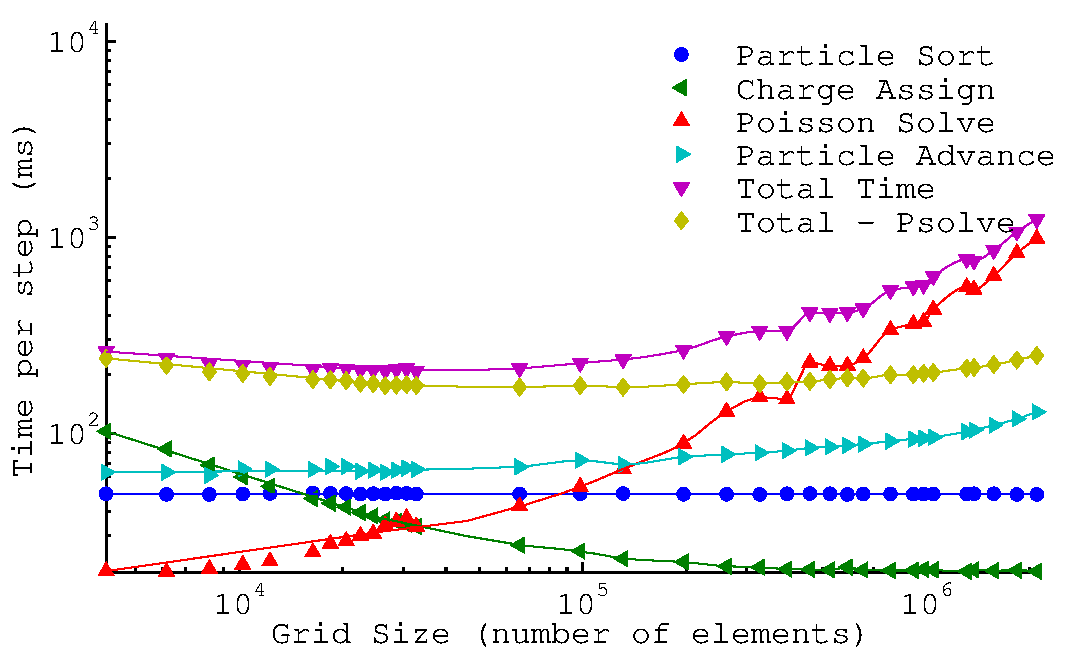
\includegraphics[width=6in]{performance/gridsize_scan34ptcls8bins.pdf}
\end{center}
\caption[Gridsize Scan with 34 million particles and $8^3$ bins.]{Gridsize Scan with 34 million particles and $8^3$ bins. Note how when the contribution from the Poisson solve is removed there is a minimum at about $10^5$ elements. }
\label{fig:grid_scan34ptcls8bins}
\end{figure}

\begin{figure}
\begin{center}
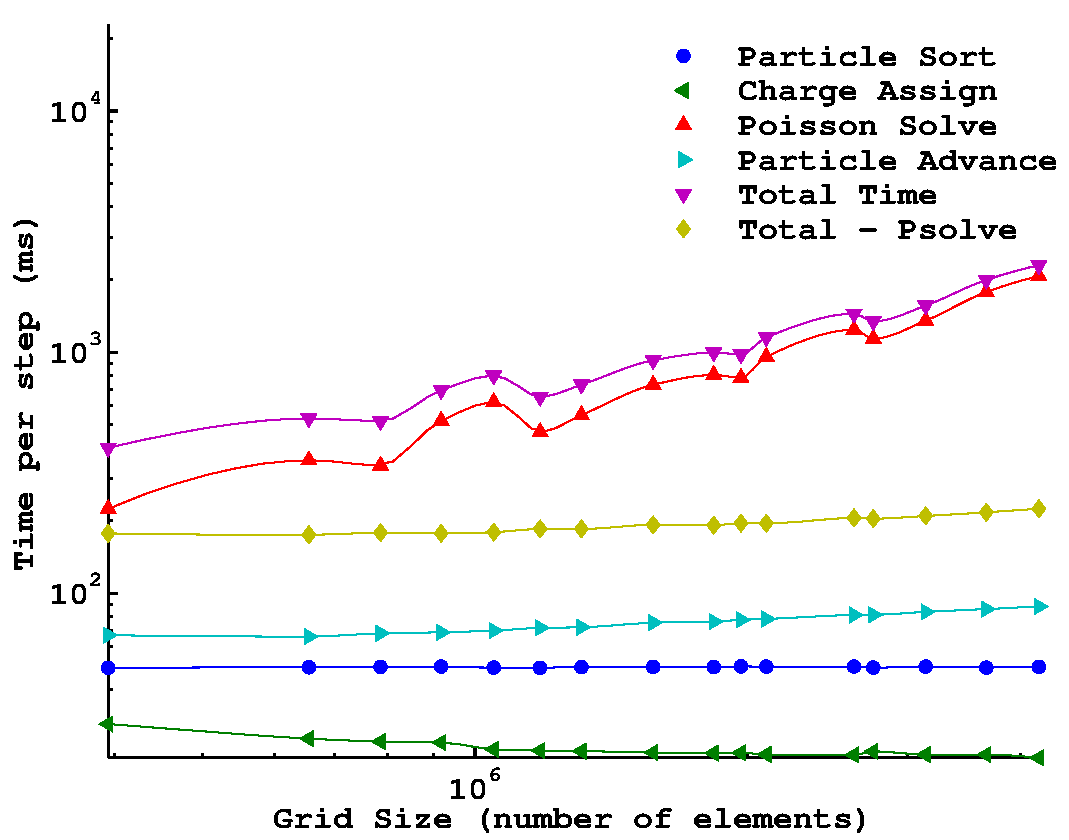
\includegraphics[width=6in]{performance/gridsize_scan34ptcls16bins.pdf}
\end{center}
\caption[Gridsize Scan with 34 million particles and $16^3$ bins.]{Gridsize Scan with 34 million particles and $16^3$ bins.}
\label{fig:grid_scan34ptcls16bins}
\end{figure}

\begin{figure}
\begin{center}
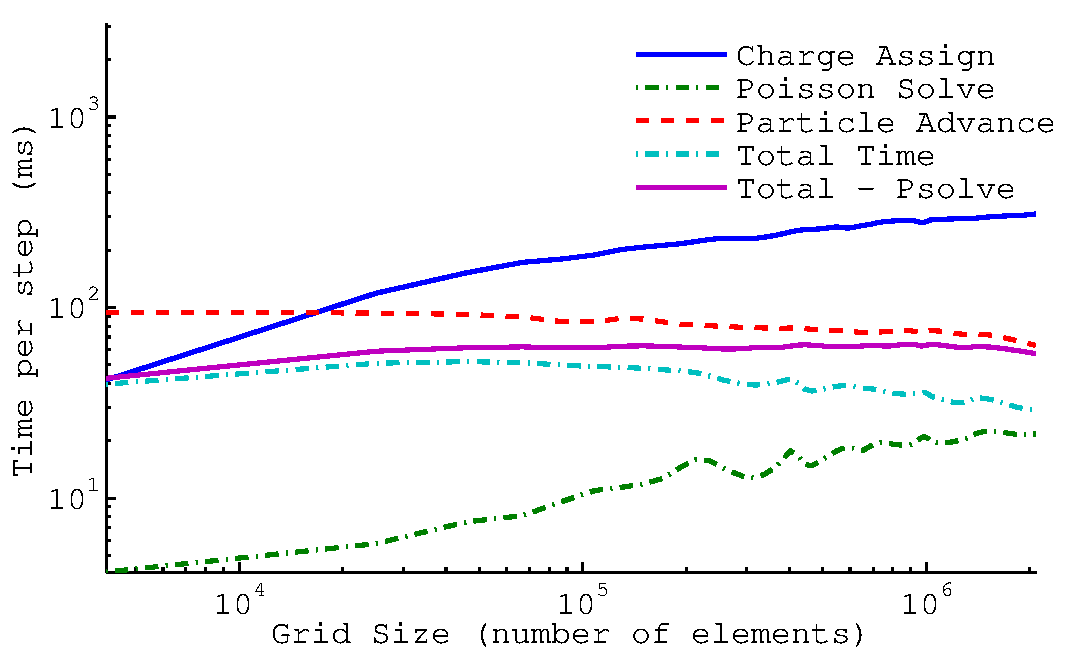
\includegraphics[width=6in]{performance/gridsize_speedup_scan.pdf}
\end{center}
\caption[Gridsize Speedup Scan with 34 million particles and $8^3$ bins]{Gridsize Speedup Scan with 34 million particles and $8^3$ bins. The total runtime is entirely dominated by the Poisson solve.}
\label{fig:grid_speedupscan}
\end{figure}

The more subtle scalings of the particle advance and charge assign can be seen in figures \ref{fig:grid_scan16ptcls8bins} through \ref{fig:grid_scan34ptcls16bins} in the cases where there are only $8^3$ bins, but do not continue their trends for $16^3$ bins. This behavior is due to the fact that these are not scalings with the absolute grid size, but rather scalings with sub-domain size. Figure \ref{fig:grid_speedupscan} shows the how much faster the GPU code is than the CPU code for various grid sizes. The GPU versions of the Poisson solve and the charge assign scale better than their CPU counterparts. However, the total runtime speedup decreases with increasing grid size. This is a result of the increased run time of the Poisson solve.

Another point of interest is the scaling of the particle sort, note that it only scales with the number of particles and is completely independent of grid size. One might expect to find some small scaling based on the distance that particles have to be moved during the sort stage, or that with fewer sub-domains the radix sort would have fewer digits to process, but this is not the case. This means that some improvement can be made to the sort, namely using the number of bins as the upper limit on the bits for the radix sort to process. Hopefully this kind of feature will be available in future releases of the \gls{gls:thrust} library.



\subsection{Threadblock Sub-Domain Size}
In chapter \ref{ch:implementation} we discussed the scaling of both the particle advance and the charge assign subroutines with grid size. Smaller grids should lead to more atomic conflicts in the charge assign and thus longer run time. On the other hand, for the particle advance smaller grids mean that a larger fraction of the grid can be stored in cache, which leads to fewer global memory accesses. Taking these two effects together, we should see a clear minimum in the data. Figure \ref{fig:subdomain_size_scan} shows the time per step of each routine vs the size of the sub-domain. Correcting for the Poisson solve we do in fact see a minimum in the run time. 

\begin{figure}[H]
\begin{center}
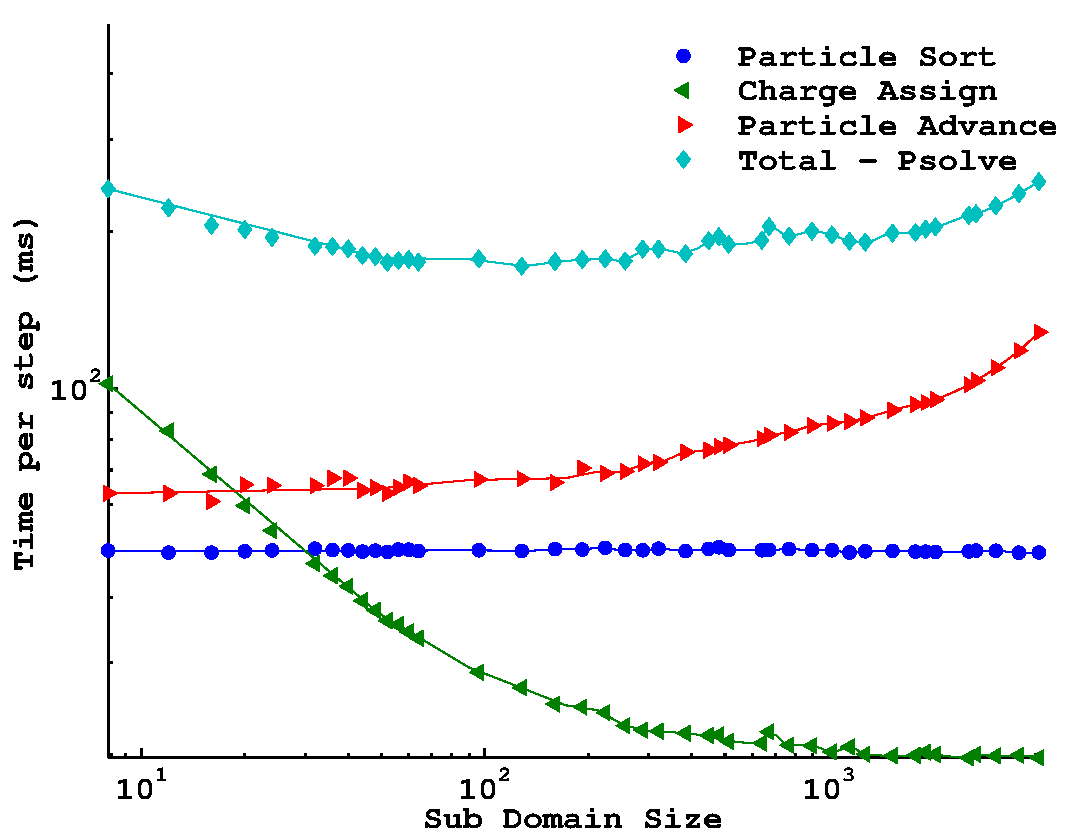
\includegraphics[width=6in]{performance/gridshape_scan.pdf}
\end{center}
\caption[Sub Domain Size scan]{Sub Domain Size scan, also known as bin size, for 34 million particles. Note the minimum in the total - psolve run time.}
\label{fig:subdomain_size_scan}
\end{figure}


	\section{Kernel Parameters Scan}
One important performance consideration for GPU computing is ensuring that every thread performs enough work to warrant the cost of its creation. For the case of the advancing kernel we adjusted the number of particles processed by each thread. This is essentially a parameter that could be optimized with through auto-tuning, and will likely vary based on the hardware configuration. We performed such a scan with the advancing kernel, ranging the number of particles processed per thread from 3 to 16. The results of this scan can can be seen in figure \ref{fig:kernel_param_scan}.

\begin{figure}[H]
\begin{center}
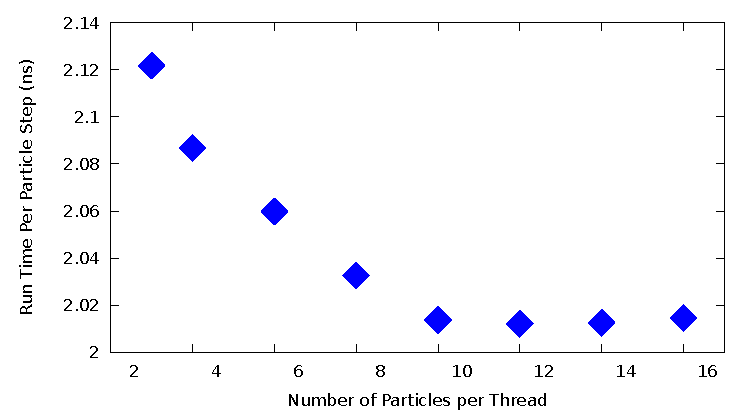
\includegraphics[width=6in]{performance/kernel_param.pdf}
\end{center}
\caption[Adjusting the amount of work per thread for the advancing kernel.]{Adjusting the amount of work per thread for the advancing kernel. Increasing the number of particle per thread has a very small effect on the runtime of the advancing kernel, although in order to run this many particles in the first place we need to run at least 2 particles per thread, since the maximum number of threads that can be launched in a single kernel is 8.3 million when using 128 threads per block.}
\label{fig:kernel_param_scan}
\end{figure}

As we can see from the figure, there is a minimum around 10 particles per thread, which is about 5\% faster than the 3 particles per thread case. This adjustment had a small, but still noticeable effect. 

%%%%%%%%%%%%%%%%%%%%%%%%%%%%%%%%%%%%
	\section{Texture Performance}
%%%%%%%%%%%%%%%%%%%%%%%%%%%%%%%%%%%%

One of the more interesting concepts that we investigated was the use of textures as a storage structure for both the potential, and the Poisson solve sparse matrix diagonals. Several comparisons between the two can be seen in figures \ref{fig:texture_tests64} and \ref{fig:texture_tests128}. These tests were performed using 42 million particles with 200 time steps on $128^3$ and $64^3$ grids. We also varied the number of cells per sorting bin (cpb) in order to determine how the performance gain from using texture memory varies with how many possible mesh points an execution block of particles can access.

\begin{figure}
\begin{center}
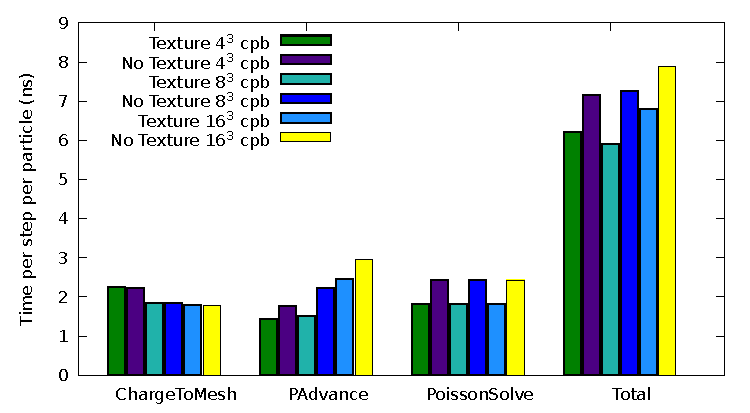
\includegraphics[width=6in]{performance/texture_tests64.pdf}
\end{center}
\caption[Comparison between texture enabled kernels on a $64^3$ grid]{Comparison between texture enabled kernels at various bin sizes. Tests used 42 million particles with 200 time steps on a $64^3$ grid.}
\label{fig:texture_tests64}
\end{figure}

\begin{figure}
\begin{center}
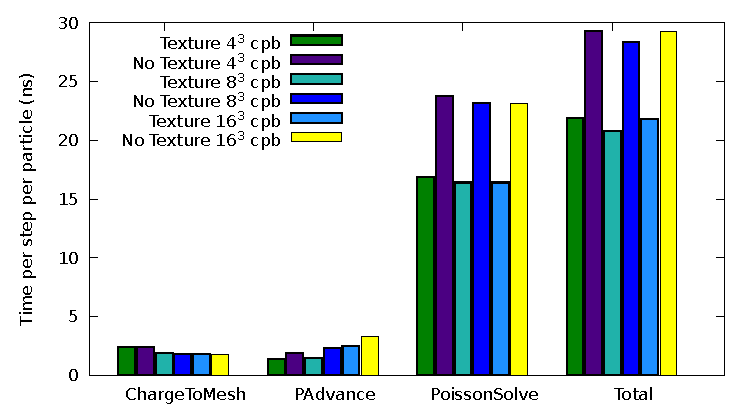
\includegraphics[width=6in]{performance/texture_tests128.pdf}
\end{center}
\caption[Comparison between texture enabled kernels on a $128^3$ grid]{Comparison between texture enabled kernels at various bin sizes. Tests used 42 million particles with 200 time steps on a $128^3$ grid.}
\label{fig:texture_tests128}
\end{figure}

As you can see from figures \ref{fig:texture_tests64} and \ref{fig:texture_tests128}, utilizing texture memory does provide a noticeable performance boost for the Poisson solve, and a small boost for the particle advance. Additionally, it is interesting to not that for particle advancing varying the number of cells per bin from $4^3$ to $8^3$ does not change the run time of the texture run. The particle advance without textures becomes slower as the number of cells per bin increases, but there is a threshold for the texture based routine.

It is likely that more data structures could be changed to textures, or surfaces for read/write data structures. The Poisson solve in particular could benefit from additional texture/surface memory usage. The primary barrier to this is not performance, but implementation difficulty. Textures are not easy to incorporate into code due to the fact that they cannot be passed as function arguments, and must be declared within the same file scope as they are used. Another downside to textures is the process of ``binding" global memory to the texture reference, which can be expensive.  

%%%%%%%%%%%%%%%%%%%%%%%%%%%%%%%%%%%%
	%\section{Resource Utilization}
%%%%%%%%%%%%%%%%%%%%%%%%%%%%%%%%%%%%
% 64^3 mesh, 40 million ptcls = 63% of time spent running kernels 200 steps

%One of the metrics used to measure the performance of GPU codes is the effective bandwidth utilization. The effective bandwidth is simply 




\chapter{Conclusion}

\section{Review}
Towards the end of chapter \ref{ch:introduction} we stated the primary goals of this project. We set out to develop a multi-GPU version of SCEPTIC3D using very generalized techniques. We came away with concrete conclusions concerning the performance impacts of using a full radix sort. We also explored ways to minimize warp divergence while handling reinjections and collisions using stream compaction and recursion. Lastly, we investigated the benefits of utilizing texture memory for constant arrays that are frequently accessed. In the end, the lessons that we learned from the exploration of each of these topics enabled us implement a GPU PIC code that attained a upwards of 100 times the performance of its CPU based counterpart. 

While the end results were impressive, we learned that a PIC code implemented on the GPU can differ greatly from the same code implemented on a CPU. Over the course of this project we analyzed the methods used by others in the development of GPU PIC implementations. The main issue that was identified by most groups was how to efficiently implement the particle to mesh step on the GPU. The conclusion that we, and many of the papers we reviewed, came to was that the particle data must be sorted in order to ensure that the majority of the accumulation can be performed using fast shared memory. So far nearly every paper that we reviewed developed their own techniques to keep the particle list sorted, with each technique optimized to fit a specific problem. 
While these specialized methods can achieve higher performance, more generalized methods tend to be easier to implement, and if they can be based on external libraries, easier to maintain. 

Some of these past works produced very generalized methods. The particle-mesh integration technique developed by Stantchev et al is a good example of a broadly applicable technique. We aimed to develop more general techniques for other steps of the PIC method. We presented a fast, very general sort based on the radix sort provided by the \gls{gls:thrust} library. While the costs associated with this sort are not negligible, the combined costs of the sort and charge assign are still comparable to the costs of the advancing step and the field solve steps. The other general technique that we developed was a way to minimize warp divergence when dealing with reinjections and collisions. The specific algorithm presented works well when the number of collisions and reinjections are small, but can be applied more generally by changing the conditions for placing a particle in a sub-list. 

The final unique property of the GPU PIC implementation presented here is the use of texture memory as the primary data structure for the potential and the backbone of the Poisson solver. We concluded that texture memory should be used as a data structure for spatially organized data. Of course there are drawbacks to texture memory, primarily that the very strict usage properties can make it difficult to integrate with the rest of the code. 



\section{Implications}
We were able to achieve speedup factors of 160 versus older CPUs and factors of 60 versus newer Intel i7 CPUs. With these speedup factors it is possible to attain cluster level performance on a multi-GPU workstation for SCEPTIC3D. In the tests we performed, we ran 50 million particles per GTX 590. There are commercially available workstations that support up to 8 graphics cards. Populated with 8x GTX 590 graphics cards, one of these workstations would be the equivalent of a 2560 core cluster for the purposes of running SCEPTIC3D. Essentially a GPU enabled SCEPTIC3D can attain cluster level performance on a single workstation. 

While we managed to improve the performance of the particle advancing and the particle-mesh interpolation steps by factors of 122 and 104 respectively, we ran into the issue where the Poisson solve became the dominant cost. As we saw in chapter \ref{ch:performance} when the grid becomes much larger than $64^3$ the cost of the Poisson solve dominates. If we start to consider even larger grid sizes, we eventually run into the limit where we are using more memory for the grid than the particle data. At that point we would have to decompose the domain across multiple GPUs such that each GPU only moved particles on part of the grid. This would greatly complicate the entire system because particles that leave one sub-domain would have to be passed from one GPU to another. Smaller PIC codes should not have to worry too much about this, although methods will have to be developed to handle this efficiently for larger codes.

One of the biggest implications of this work is its effect on the particle sorting step. Previous groups attempted to solve the sorting question using the radix sort implementation provided by the CUDPP library. However, this implementation was unacceptably slow, and combined with the poor memory access patterns of older cards, the library sort was out of the question. Recently the radix sort, now provided by the \gls{gls:thrust} library, has been significantly improved. This fact, combined with the improved memory access patterns has resulted in a radix based particle sort method with significantly better performance. The performance of the \gls{gls:thrust} sort is currently good enough that there is little reason to develop a specialized sorting technique. 

\section{Future Work}
Within the scope of the GPU implementation of SCEPETIC there is at least one additional physics component that has not yet been included due to time constraints, the collision operator. While we have laid out the framework for implementing collisions on the GPU we have not yet implemented the entirety of that framework. Additionally, the re-injection particle list is currently calculated on the CPU, and a portion of this 'pool' is transfered to the GPU during the re-injection phase. Refilling the particle list on the CPU currently costs about 1/3\textsuperscript{rd} the cost of the particle advance. Implementing this on the GPU would significantly reduce the cost of this step, as well as eliminate the particle list transpose and host to device memory copy currently required. Further improvements to SCEPTIC3D could be made by optimizing the advancing kernel, specifically optimizing the force interpolation function to require fewer registers. 

Pertaining to GPU PIC implementations in general, more work needs to be done concerning large grid sizes. As previously stated, two of the major issues facing larger scale GPU PIC implementations are multi-GPUs domain decomposition and optimizing large field solves. Developing asynchronous techniques that perform computations on both the GPU and CPU simultaneously is another high priority. 




\appendix
\chapter{Tables}

\begin{center}
\begin{table}
\begin{tabular}{| p{4.0cm} | p{3.5cm} |}
\hline
Component & Runtime (ms) \\ \hline
Particle data read, move, and write & 375 \\ \hline
Potential Grid Read & 467 \\ \hline
Charge Assign & 1.143e4  \\ \hline
Total & 1.227e4  \\ \hline
\end{tabular}
\caption{Total Execution times for 100 iterations of the key steps of the move kernel at three different optimizations.}
\label{tab:GPUPIC_basetime} 
\end{table}
\end{center}


\noindent \begin{table}
\begin{tabular}{| p{4.0cm} | p{3.5cm} | p{3.5cm} |}
\hline
Component & Atomic-Updates (ms) & Sorted+Reduction (ms) \\ \hline
Particle data read, move, and write & 375 & 468 \\ \hline
Potential Grid Read & 467 & 285 \\ \hline
Charge Assign & 1.143e4 & 542 \\ \hline
Particle List Sort & 0 & 2.305e3 \\ \hline
Total & 1.227e4 & 3600 \\ \hline
\end{tabular}
\caption{Total Execution times for 100 iterations of the key steps of the move kernel at two different optimizations.}
\label{tab:GPUPIC_comparison}
\end{table}

\noindent \begin{table}[h]
\begin{tabular}{| p{4.0cm} | p{3.5cm} | p{2.5cm} | p{4.0cm} |}
\hline
Component & SoA (ms) & AoS (ms) & Speedup (SoA vs AoS) \\ \hline
Particle data read, move, and write & 758 & 955 & 1.26x \\ \hline
Count Particles & 32.7 & 109 & 3.35x \\ \hline
Data Reorder & 346 & 480 & 1.38x \\ \hline
Total CPU run time & 2491 & 3284 & 1.31x \\ \hline
\end{tabular}
\caption{Execution times of main steps for Array of Structures and Structure of Arrays. Count Particles and Data Reorder are steps used for a sorted particle list. Count Particles counts the number of particles in each sub-domain. Data Reorder reorders the particle list data after the binindex / particle ID pair have been sorted by the radix sort.}
\label{tab:struct_compare} 
\end{table}


\noindent \begin{table}[h]
\begin{tabular}{| p{4.0cm} | p{3.5cm} | p{2.5cm} | p{4.0cm} |}
\hline
Component & CPU (ns) & GPU (ns) & Speedup \\ \hline
Sort & 0 & 1.240 & - \\ \hline
Charge Assign & 192.055 & 0.621 & 308x \\ \hline
Charge Assign \& Sort & 192.055 & 1.846 & 104x \\ \hline
Poisson Solve & 38.398 & 1.896 & 21x \\ \hline
Particle Advance & 185.245 & 1.520 & 122x \\ \hline
Total\footnote[1] & 417.519 & 5.919 & 71x \\ \hline
\end{tabular}
\caption{CPU and GPU Runtime comparison for 2 GTX 470's vs an Intel(R) Core i7 930 Test was performed using 2 MPI threads handling 21 million particles each on a $64^3$ grid.}
\label{tab:speedup} 
\end{table}

\noindent \begin{table}[h]
\begin{tabular}{| p{4.0cm} | p{3.5cm} | p{2.5cm} | p{4.0cm} |}
\hline
Component & CPU (ns) & GPU (ns) & Speedup \\ \hline
Sort & 0 & 1.272 & - \\ \hline
Charge Assign & 312.210 & 0.802 & 389x \\ \hline
Charge Assign \& Sort & 312.210 & 2.075 & 150x \\ \hline
Poisson Solve & 637.349 & 5.393 & 118x \\ \hline
Particle Advance & 391.335 & 2.325 & 168x \\ \hline
Total\footnote[1] & 1352.461 & 12.958 & 104x \\ \hline
\end{tabular}
\caption{CPU and GPU Runtime comparison for a GTX 590 vs an Intel(R) Xeon(R) CPU E5420. Test was performed using 2 MPI threads handling 17 million particles each on a $64^3$ grid.}
\label{tab:speedup2} 
\end{table} 




\clearpage
\newpage

%\chapter{System Bandwidth Comparison}


In figures \ref{fig:speedup} and \ref{fig:speedup2} we presented an overview for performance of the GPU version of SCEPTIC3D on two distinct systems. System 1 consisted of an Intel(R) Core i7 930 quad core processor clocked at 2.8GHz and two EVGA GTX 470 graphics cards. System 2 consisted of two Intel(R) Xeon(R) E5420 quad core processors clocked at 2.53GHz and one EVGA GTX 590. In figure \ref{fig:speedup2} the speedup factors for the GPU version vs the CPU version were much higher on system 2. There are two reasons for this. The first reason is that the GPU in system 2, the GTX 590, is more powerful than the two GTX 470's in system 1. The second reason has to do with the difference in memory bandwidth between the two systems.

\noindent \begin{figure}
\begin{center}
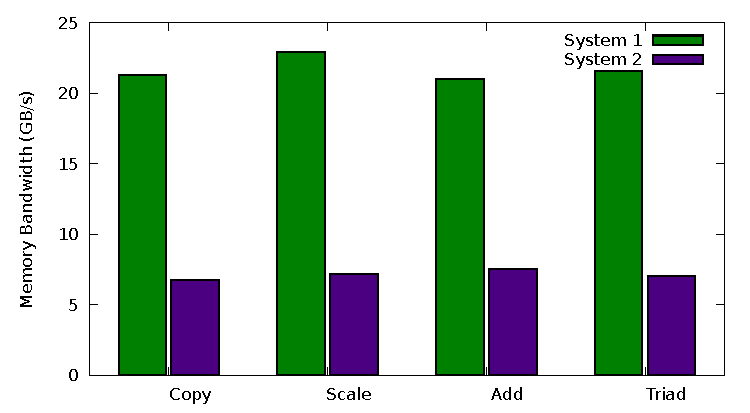
\includegraphics[width=6in]{appb/bandwidth_test.pdf}
\end{center}
\caption[System Memory Bandwidth Comparison]{System memory bandwidth comparison for the two test systems used to generate the results in \ref{fig:speedup} and \ref{fig:speedup2}.}
\label{fig:memory_bandwidth_compare} 
\end{figure} 

In figure \ref{fig:memory_bandwidth_compare} we performed four vector operations on 20 million element arrays. These vector operations consisted of a simple copy $B = A$, a scalar multiply $B = \alpha A$, a vector add $C = A+B$, and a triad $C = B+\alpha A$. MPI was used to run one copy of the each operation for every core on the target system, the MPI threads were synchronized between operations. Run times were recorded for 50 iterations of the vector operations, the run time at each iteration is the mean of the individual thread run times. The memory bandwidth of each operation is calculated as the number of bytes read and written divided by the minimum run time.    



\clearpage
\newpage

%% This defines the bibliography file (main.bib) and the bibliography style.
%% If you want to create a bibliography file by hand, change the contents of
%% this file to a `thebibliography' environment.  For more information 
%% see section 4.3 of the LaTeX manual.
\begin{singlespace}
\bibliography{main}
\bibliographystyle{plain}
\end{singlespace}

\end{document}

